\documentclass[11pt,a4paper]{article}

% Basic packages
\usepackage[fontset=fandol]{ctex}
\usepackage{amsmath, amssymb}
\usepackage{graphicx}
\usepackage[margin=2.15cm]{geometry}
\usepackage[most]{tcolorbox}
\usepackage{etoolbox}
\usepackage{listings}
\usepackage{hyperref}
\usepackage{booktabs}
\usepackage{subcaption}
\usepackage{float}
\usepackage{tikz}
\IfFileExists{pgfplots.sty}{
    \usepackage{pgfplots}
    \pgfplotsset{compat=1.18}
}{}

% Highlight box palette: low-saturation and print-friendly.
% Visual weight is ordered by teaching role, so a page mixing several boxes still
% reads important > warning > knowledge > dialogue instead of competing for attention.
% Title text is white on every title bar; contrast stays within WCAG AA (4.5:1--6.0:1).
\definecolor{kbBack}{HTML}{F2F6FA}\definecolor{kbFrame}{HTML}{9DB4CC}\definecolor{kbTitle}{HTML}{52708F}
\definecolor{ibBack}{HTML}{FBF5E7}\definecolor{ibFrame}{HTML}{C9A961}\definecolor{ibTitle}{HTML}{7D5F1E}
\definecolor{wbBack}{HTML}{FCF2F0}\definecolor{wbFrame}{HTML}{D6A096}\definecolor{wbTitle}{HTML}{9E4F43}
\definecolor{dbBack}{HTML}{F4F7F3}\definecolor{dbFrame}{HTML}{AEC2AC}\definecolor{dbTitle}{HTML}{5F7F64}

\tcbset{softbox/.style={
    enhanced, boxrule=0.8pt, arc=2pt, left=3mm, right=3mm, top=2mm, bottom=2mm,
    coltitle=white, fonttitle=\bfseries, toptitle=0.6mm, bottomtitle=0.6mm
}}

% Highlight boxes
\newtcolorbox{knowledgebox}[1]{
    softbox, colback=kbBack, colframe=kbFrame, colbacktitle=kbTitle, title=#1
}

\newtcolorbox{importantbox}[1]{
    softbox, colback=ibBack, colframe=ibFrame, colbacktitle=ibTitle, title=#1
}

\newtcolorbox{warningbox}[1]{
    softbox, colback=wbBack, colframe=wbFrame, colbacktitle=wbTitle, title=#1
}

\newtcolorbox{dialoguebox}[1]{
    softbox, breakable, colback=dbBack, colframe=dbFrame, colbacktitle=dbTitle, title=#1
}

% Listings
\lstset{
    language=Python,
    basicstyle=\ttfamily\small,
    keywordstyle=\color{blue},
    stringstyle=\color{red!60!black},
    commentstyle=\color{green!60!black},
    breaklines=true,
    frame=single,
    numbers=left,
    numberstyle=\tiny\color{gray},
    captionpos=b,
    extendedchars=false
}


\usepackage{tabularx}
\newcolumntype{L}[1]{>{\raggedright\arraybackslash}p{#1}}
\usetikzlibrary{positioning}
\hypersetup{colorlinks=true,linkcolor=kbTitle,urlcolor=kbTitle,pdftitle={CMU L2 工具使用：中文课程讲义},pdfauthor={Based on Graham Neubig; Chinese notes prepared with Codex}}
\renewcommand{\baselinestretch}{1.13}
\setlength{\parskip}{.4em}
\setlength{\emergencystretch}{2em}
\setcounter{tocdepth}{1}
\lstset{basicstyle=\ttfamily\footnotesize,columns=fullflexible,keepspaces=true,xleftmargin=6mm,framexleftmargin=4mm}
\begin{document}
\special{pdf:minorversion 7}
\hypersetup{pageanchor=false}
\begin{titlepage}
\centering
\vspace*{.9cm}
{\Large CMU 11-768 · AI Agents\par}
\vspace{.6cm}
{\Huge\bfseries 语言模型 Agent 的工具使用\par}
\vspace{.4cm}
{\Large 从调用协议到可靠执行\par}
\vspace{.5cm}
{\large L2 中文课程讲义\par}
\vspace{1cm}
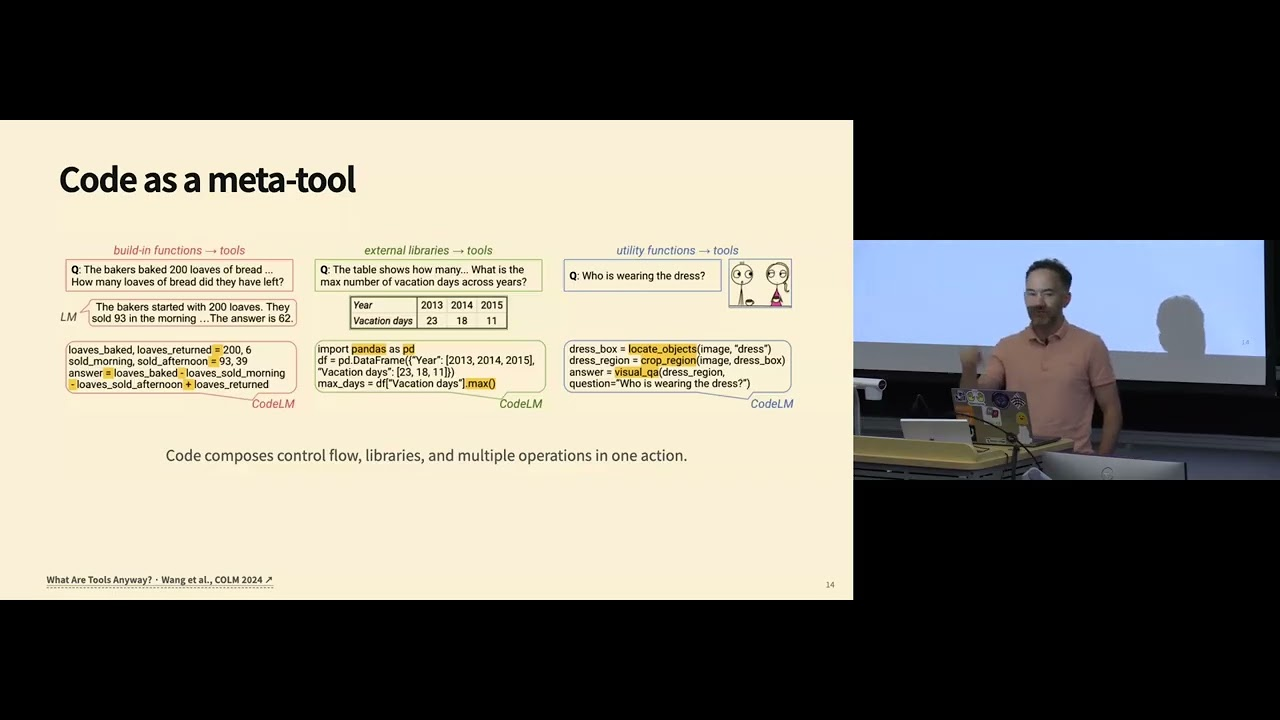
\includegraphics[width=\textwidth]{figures/原视频封面.jpg}\par
{\small 图：原视频封面\par}
\vfill
\begin{tcolorbox}[colback=kbBack,colframe=kbFrame,width=\textwidth]
\textbf{主讲 / 频道}：Graham Neubig\par
\textbf{课程}：Carnegie Mellon University，11-768 AI Agents，Fall 2026\par
\textbf{时长}：57 分 22 秒\par
\textbf{整理日期}：2026 年 10 月 2 日\par
\textbf{原视频}：\href{https://www.youtube.com/watch?v=jXChFB4JSyw}{youtube.com/watch?v=jXChFB4JSyw}
\end{tcolorbox}
\end{titlepage}
\pagenumbering{arabic}
\hypersetup{pageanchor=true}
\section*{本讲概览}
本讲说明语言模型怎样通过工具取得新信息、执行计算与改变应用状态。内容从工具与程序化调用开始，逐步展开消息模板、模型协议、派发执行、约束解码、REST 与 MCP、并发调度，以及工具使用的多层评价。结束时将这些机制归纳为一套相互连接的运行系统。

讲义依据课程口述、带时间转录、官方课件与视频画面整理。图注分别标明课件页码、口述区间或实际截帧时间。官方课件中的额外展开注明为课件补充；重写代码、数学形式化与归纳图注明为教学解释。接口代码按课堂展示范围说明其作用。
\tableofcontents

\clearpage
\section{工具如何扩展语言模型的能力}
\subsection{让 token 预测连接外部程序}
语言模型能够生成一个问题的回答，也能够生成一段程序，但外部世界不会因为这段文本出现就自动改变。要查询网页、取得账户数据、运行程序或操作应用，需要有软件接收请求并实际执行。本讲把这个接口称为工具。

\begin{importantbox}{工具的定义}
工具是语言模型可以借助它调用外部计算机程序的接口。模型提出调用请求，外部软件决定是否执行以及怎样执行。搜索、计算器、浏览器、Python 和应用 API 都可以承担这种接口。
\end{importantbox}

这个定义保持了两个职责之间的关系。模型负责生成行动表达，工具与运行系统负责把表达连接到真实计算或环境操作。工具调用可以遵循较统一的消息机制，调用之后发生的事却很不同：搜索返回文本，计算器返回数值，图像工具返回图像，账户接口可能读取私人状态或改变外部系统。

\subsection{扩展能力与辅助能力}
课程将收益分为两类。\textbf{扩展（extend）}让模型取得参数中没有的信息，或执行原本无法通过文本生成完成的动作。\textbf{辅助（facilitate）}把模型原则上能够处理的工作交给更快、更可靠的程序。

例如，一个只靠冻结参数的模型无法直接知道训练之后刚发生的事件；查询工具能取得新证据。另一方面，模型可以通过推理完成乘法，但两个七位数的乘法可能需要生成很多推理内容，计算器可以迅速完成。这两类收益有时同时出现：程序既带来可执行计算能力，也能提高准确性和效率。

\begin{center}\small
\renewcommand{\arraystretch}{1.25}
\begin{tabularx}{\textwidth}{L{2.5cm} L{3.1cm} X}
\toprule
需求 & 典型工具 & 提供的收益\\
\midrule
当前信息 & 搜索 & 取得新证据，支持回答中的事实判断。\\
精确计算 & 计算器或 Python & 通过实际执行得到更可靠、通常也更快的结果。\\
私人状态 & 账户 API & 在授权下取得当前应用或账户的数据。\\
外部行动 & 浏览器或 API & 操作环境，例如创建记录或改变应用状态。\\
\bottomrule
\end{tabularx}
\end{center}

官方课件还补充了一项设计原则：只有工具收益超过其延迟、成本、失败机会和风险时，才值得调用。工具增加了可做的事，也增加了需要处理的执行环节。

\begin{figure}[H]\centering
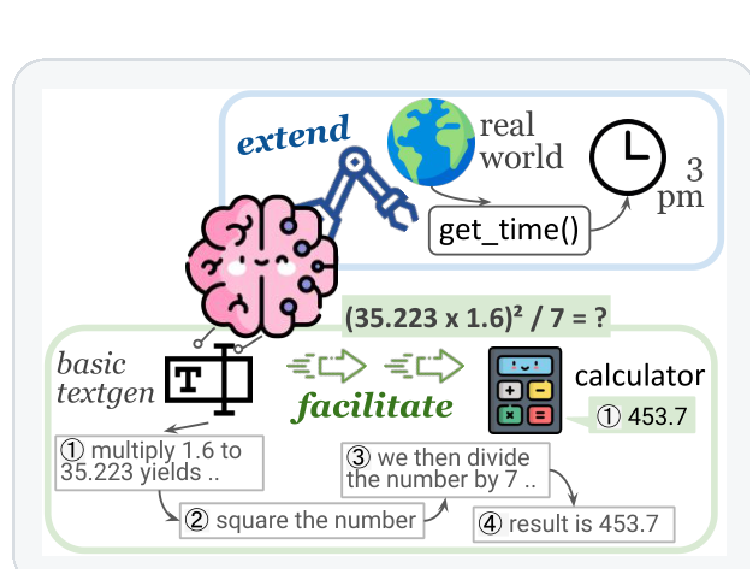
\includegraphics[width=.68\textwidth]{figures/工具扩展与辅助.pdf}
\caption{工具既能接触外部信息，也能将计算交给程序。\protect\footnotemark}
\end{figure}
\footnotetext{官方课件第 4 页裁图；对应口述 00:01:09--00:03:33。}

\subsection{从面向用户的能力推导工具接口}
课堂通过 ChatGPT 类应用讨论工具种类：先确定希望应用提供哪些能力，再为每类交互定义接口。下面的例子是课程中的示意调用，用于说明接口如何承接这些能力。

\paragraph{文本回答与结束任务。}
文字回答可以由一个 \texttt{finish(text)} 控制动作结束 Agent 循环，也可以让运行系统在模型没有请求工具时结束。这两种方式改变的是控制流程。官方课件专门注明：\texttt{finish} 是 harness 的控制动作，不属于外部程序工具。把二者区分开，既能解释课堂为什么将回答放进能力列表，也能保持工具定义清楚。

\paragraph{检索与生成。}
\texttt{search\_web(query)} 获取网页信息，模型再以结果为依据回答。示意任务是查询 CMU 当天公告。讲者回应“RAG 已过时”的说法时强调，先检索上下文、再利用上下文生成的过程已经普遍融入应用，因而常常不再被单独点名。

这里的教学联系是：检索增强生成描述了信息如何支持生成，而 Agent 的工具调用描述了谁在何时选择并执行检索。一个固定流水线可以总是检索；一个 Agent 也可以在任务中根据需要发起查询。二者可以结合。

\begin{figure}[H]\centering
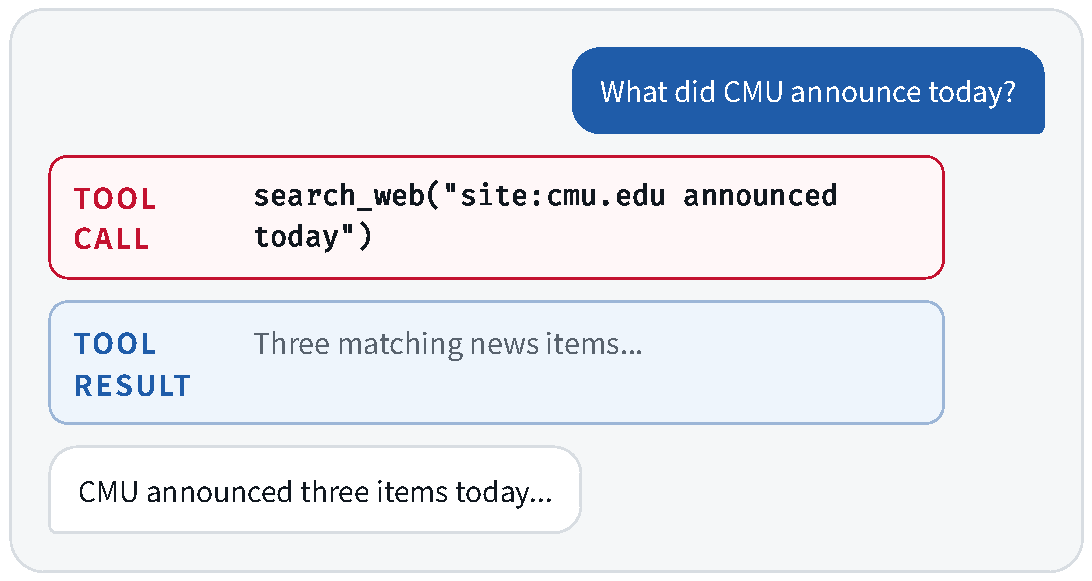
\includegraphics[width=.82\textwidth]{figures/检索调用与结果.pdf}
\caption{检索工具先返回信息，模型再依据结果生成回答。\protect\footnotemark}
\end{figure}
\footnotetext{官方课件第 9 页裁图；对应口述 00:07:11--00:08:29。}

\paragraph{执行代码。}
\texttt{execute\_code(code)} 在隔离环境中运行程序并返回输出。官方例子计算 18、23、41、54 的平均数：

\noindent\begin{minipage}{\textwidth}
\begin{lstlisting}[language=Python,caption={课程代码执行示例：生成请求、实际计算与返回结果}]
execute_code("sum([18,23,41,54])/4")
# Tool result: 34.0
\end{lstlisting}
\end{minipage}

模型随后可以把返回值组织成“平均数为 34”的回答。执行程序和口头解释计算结果分别由程序环境与语言模型承担。

\paragraph{生成图像。}
\texttt{generate\_image(query)} 接收文字描述并返回图像资产。课件例子是水彩风格的机器人在图书馆学习。讲者指出，决定传给图像模型的描述也是工具使用的一部分：语言模型可能把用户短指令扩写成更详细的生成提示。

课件给出的是一个简短的描述示例。讲者对提示扩写的讨论进一步说明，选择工具之外还需要组织工具的输入，描述中的风格、主体和场景都可能影响结果。

\begin{figure}[H]\centering
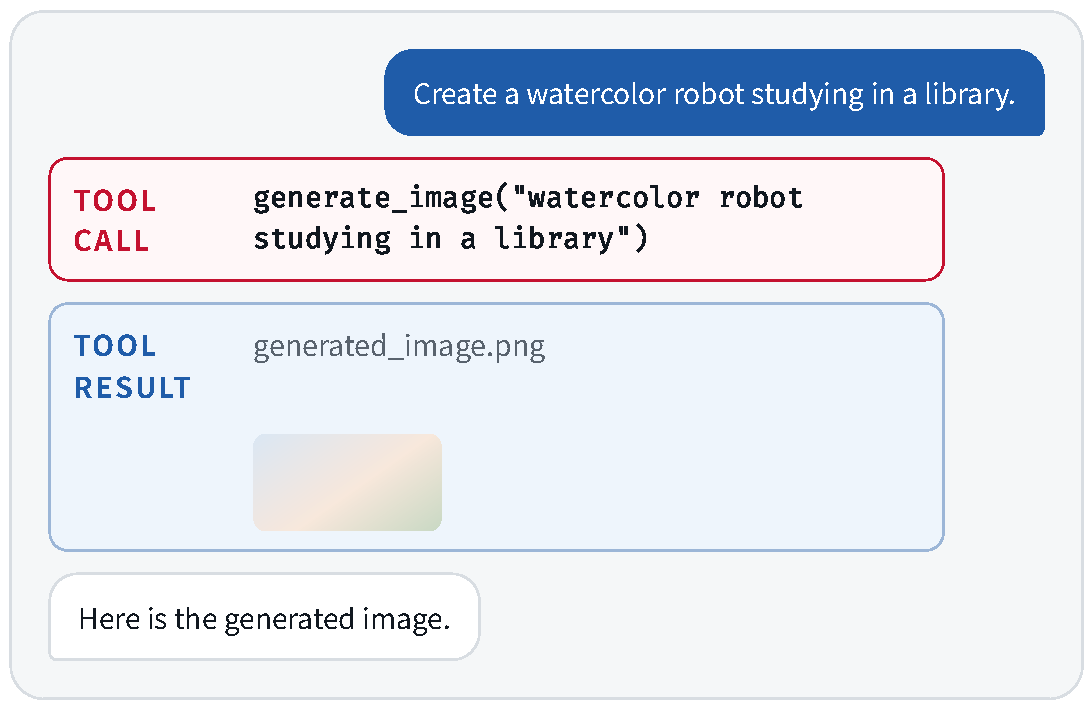
\includegraphics[width=.78\textwidth]{figures/图像生成调用.pdf}
\caption{工具输入是文字描述，返回的能力可以是图像资产。\protect\footnotemark}
\end{figure}
\footnotetext{官方课件第 11 页裁图；对应口述 00:08:29--00:09:53。}

\paragraph{应用专用接口。}
\texttt{create\_grocery\_cart(items)} 为特定应用提供创建购物车的能力。课件中的参数是香蕉、牛奶和咖啡，返回内容包含购物车标识 C17、3 件商品和 \$31.42。这个示意调用创建了购物车；它没有展示支付成功或完成购买，不能把二者写成同一结果。

课堂还讨论了 Blender、LaTeX 与 Slack 等能力。生成 Blender 场景并渲染、把 LaTeX 编译成 PDF，或与 Slack API 交互，都涉及外部执行。若界面只是把已有公式显示出来，则可能只是前端渲染。能力名称相似，底层是否执行外部程序仍需具体判断。

\begin{knowledgebox}{以能力需求选择接口}
先确定需要取得哪类信息或完成哪项行动，再决定工具接口。查网页、执行程序、生成图像和操作账户具有不同输入、返回值与副作用，不能仅因为它们都采用工具调用消息就视为相同能力。
\end{knowledgebox}

\subsection{本章小结}
工具把模型生成的请求接到外部程序。它既能扩展模型的信息与行动范围，也能把耗时或容易出错的工作交给程序完成。设计时需要明确接口的收益、结果和副作用，并区分任务结束这样的控制动作与真实外部执行。

\clearpage
\section{程序化工具调用：用代码组合多步行动}
\subsection{为什么代码可以成为元工具}
一种做法是给模型提供几十个 API，让它在每轮选择其中一个调用；并行调用也可以一次发出多个独立请求。复杂任务还会涉及中间变量、重复操作、结果汇总和分支。代码能够把这些结构表达在一次可执行请求中，因此课程将它称为\textbf{元工具（meta-tool）}。

程序可以使用内置运算、导入外部库，并调用应用提供的函数。执行器接收一段代码，就能够执行其中组织好的多次操作。模型与执行器之间的往返次数可能减少，但程序内部实际调用的 API 不一定减少。

\begin{importantbox}{代码组织控制流与数据流}
程序化工具调用把多个操作及其依赖关系写进代码。循环表达重复，变量保存中间结果，库和专用函数提供既有能力。一次代码动作可以组合多次底层调用。
\end{importantbox}

\subsection{三种组成方式}
官方 P14 用三组例子说明代码怎样整合工具。

第一组是内置运算。面包示例代码把烘焙量、退回量、上午与下午销量存入变量，再用减法和加法组合得到结果。按可见代码的数值作教学重写：200 减去 93 和 39，再加上退回的 6，结果为 74。它说明了代码的作用：模型表达数值关系，程序执行具体运算。

第二组是库调用。课件导入 pandas，构造包含 2013、2014、2015 年及 23、18、11 天休假的表格，再调用最大值函数：

\noindent\begin{minipage}{\textwidth}
\begin{lstlisting}[language=Python,caption={根据课程 P14 重排的代码：用 pandas 取得休假天数最大值}]
import pandas as pd

df = pd.DataFrame({
    "Year": [2013, 2014, 2015],
    "Vacation days": [23, 18, 11],
})
max_days = df["Vacation days"].max()
print(max_days)  # 23
\end{lstlisting}
\end{minipage}

导入库使程序能够使用库提供的能力。模型无需通过自然语言手算表格中的所有操作，也无需让 Agent 运行系统分别暴露每个 pandas 方法为独立的 JSON 工具。

第三组是应用专用函数。图中的视觉问答先用 \texttt{locate\_objects} 定位裙子，再以 \texttt{crop\_region} 裁剪，最后用 \texttt{visual\_qa} 判断穿裙子的人。这个例子展示的是数据流：前一步的返回值直接成为下一步输入。

\begin{figure}[H]\centering
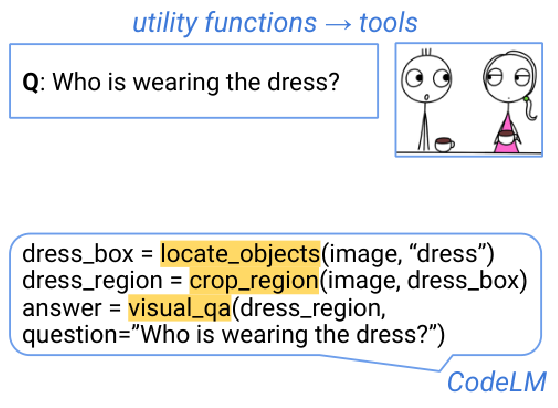
\includegraphics[width=.62\textwidth]{figures/视觉问答的工具组合.pdf}
\caption{视觉问答中的组合：定位对象、裁剪区域、调用问答接口。\protect\footnotemark}
\end{figure}
\footnotetext{官方课件第 14 页裁图；对应口述 00:10:27--00:12:37。}

\subsection{CodeAct：把逐个调用改为程序组合}
CodeAct 的示意任务是比较美国、日本、德国和印度，找出购买手机型号“CodeAct 1”的最低总成本。可用接口提供汇率与税率、当地价格、换汇加税、运费及最终价格估计。

文本或 JSON 方式可以逐步查询：先看德国汇率和税率，再查手机价格，再换汇加税，随后重复其他国家。每一步都可能成为模型与执行器之间的一次交互。

代码方式可以用一个循环组织整个比较。下面按课件结构教学重写，统一图中不一致的手机型号名，并将这些函数视为执行环境预先提供的接口。

\noindent\begin{minipage}{\textwidth}
\begin{lstlisting}[language=Python,caption={CodeAct 课件示例的教学重写：组合四个国家的价格查询}]
countries = ["USA", "Japan", "Germany", "India"]
final_prices = {}

for country in countries:
    exchange_rate, tax_rate = lookup_rates(country)
    local_price = lookup_phone_price("CodeAct 1", country)
    converted_price = convert_and_tax(
        local_price, exchange_rate, tax_rate
    )
    shipping_cost = estimate_shipping_cost(country)
    final_prices[country] = estimate_final_price(
        converted_price, shipping_cost
    )

best_country = min(final_prices, key=final_prices.get)
print(best_country, final_prices[best_country])
\end{lstlisting}
\end{minipage}

循环负责重复流程，字典保存每个国家的结果，\texttt{min} 从已有程序库中完成比较。官方图给出的示意结论是日本、904 美元，数值属于论文的示意任务。运行上面的代码需要实际接口及它们的数据，当前代码块本身不包含这些实现。

这里的效率来自\textbf{操作组合}。一次提交代码不等于只调用一次外部 API，也不保证其内部请求已经并行。程序按所写控制流执行，执行环境仍需处理权限、错误与资源使用。

\subsection{实验结果支持什么}
课程用 CodeAct 结果比较三种动作表示：Code、JSON 和 Text。左图是任务成功率，右图是平均交互轮数。图中展示了 8 个模型，包括两种 GPT-4、两种 GPT-3.5、Claude 2、Gemini Pro、text-davinci-003 和 Llama-2-70B-chat。

官方课件明确写出：在展示的 8 个模型中，代码动作在 8/8 上取得最高成功率，在 7/8 上使用最少交互轮数；在研究全部 17 个模型中，这两项计数分别都是 12/17。\texttt{text-davinci-003} 是图中轮数优势的例外，其代码方式的平均交互轮数略多于 JSON。

这些结果支持在该研究设置中，代码能够改善许多工具任务的成功率，并常常减少交互轮数。讲者强调，收益也出现在原本被视为普通工具使用、并非传统代码题的任务中。结果不能推广成“所有模型与任务均应采用代码”，也不能从交互轮数直接换算出完整运行时间、价格或风险。

\begin{figure}[H]\centering
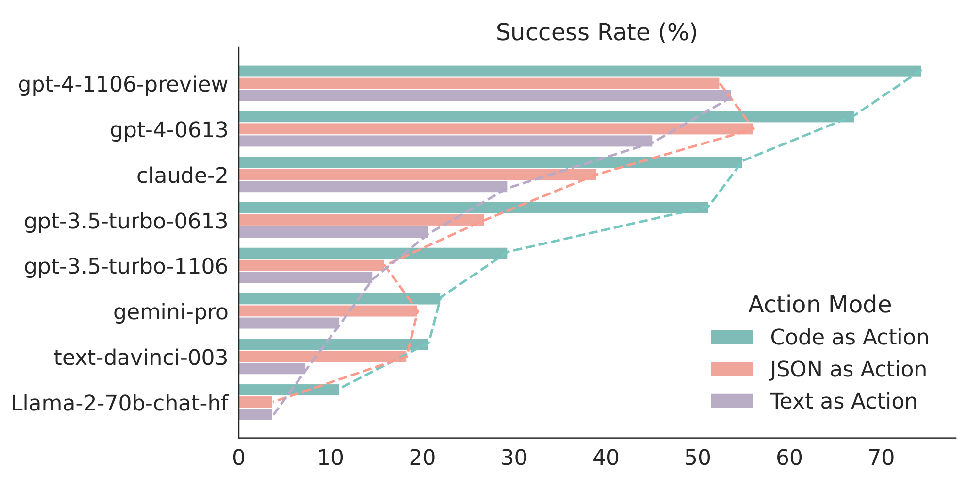
\includegraphics[width=.98\textwidth]{figures/CodeAct_成功率.pdf}
\caption{CodeAct 成功率对比；保留原图模型、动作模式与百分比轴。\protect\footnotemark}
\end{figure}
\footnotetext{官方课件第 16 页左图；对应口述 00:13:07--00:14:18。}

\begin{figure}[H]\centering
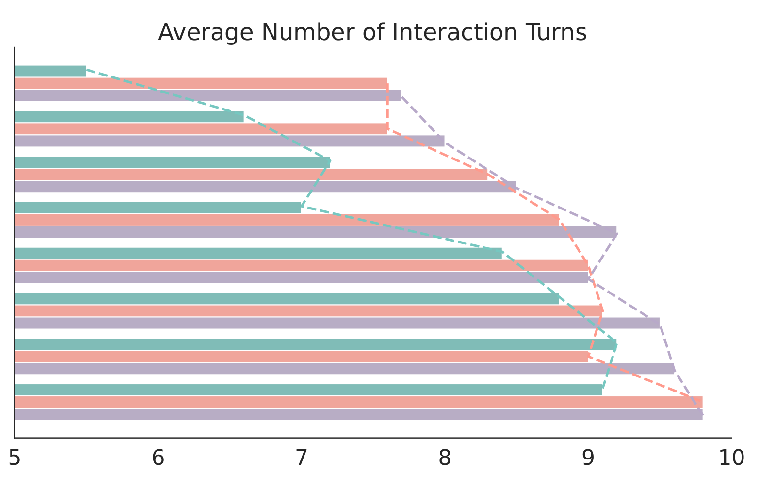
\includegraphics[width=.83\textwidth]{figures/CodeAct_交互轮数.pdf}
\caption{平均交互轮数；模型的行序与上一图相同，颜色含义也相同。\protect\footnotemark}
\end{figure}
\footnotetext{官方课件第 16 页右图；对应口述 00:13:07--00:14:18。}

\begin{warningbox}{表示能力更强，约束也更难}
代码允许循环、变量、库调用和多步组合，也可能产生无限循环、使用受污染的依赖，或消耗大量内存、磁盘与 CPU。减少交互轮数并不消除这些风险。
\end{warningbox}

\subsection{表达力为何带来执行边界问题}
讲者从循环开始讨论：模型可能生成无限循环，执行系统必须能处理它。库还带来版本与安全问题；被污染的依赖会将风险传递到 Agent 的执行环境。广泛的动作空间也使验证更难，模型可以同时操作文件、网络或进程，产生比窄接口更复杂的后果。

因此，程序化工具调用需要结合沙箱、资源限制和权限。官方课件第 17 页 还列出审计日志。根据这些机制的教学归纳是：窄的有类型函数更容易限定允许的动作；代码适合表达复杂组合；选择取决于任务需要的表达力，以及运行系统能落实的执行边界。

\subsection{本章小结}
代码将工具组合成可执行的控制流与数据流。CodeAct 展示了这种表示在多种工具任务上的收益，同时也保留了明确适用范围。接口越能表达复杂行动，运行系统越需要处理循环、依赖、资源和权限。

\clearpage
\section{工具调用如何成为模型的输入与输出}
\subsection{文本输出与行动请求都可以由 token 表达}
模型本身继续预测 token。普通输出可以是“The weather is sunny.”，工具输出则可以包含表示调用边界的标记和 \texttt{get\_weather(...)}。外部系统识别这些内容后执行请求。

\noindent\begin{minipage}{\textwidth}
\begin{lstlisting}[language={},caption={课程工具输出示意：调用标记表达请求边界}]
<tool_call>
get_weather(...)
</tool_call>
\end{lstlisting}
\end{minipage}

这些标记只是示意格式，不能视为所有模型通用的协议。讲者还在板书中说明，一次生成可以包括推理、给用户看的消息和工具调用。它们承担不同作用：推理用于继续生成，消息帮助用户了解过程，调用则请求执行具体行动。

讲者说推理与行动可以组织在一个 completion 中，这描述的是模型输出结构。真正的 ReAct 环境循环仍然需要 harness：执行调用、获得观察，再让模型继续生成。一次文本生成不会自行完成文件访问或 API 请求。

\subsection{工具标记可以在后续训练阶段引入}
课堂问题问到，工具调用标记是否必须在预训练开始时已经存在于模型词表中。讲者先回答“是”，随后纠正：在大规模互联网预训练时未必需要它们，更常见的是在中间训练（mid-training）阶段引入并学习目标格式，之后还可能继续强化学习。

\begin{importantbox}{以讲者修正后的回答为准}
工具格式需要模型能够表示并学会使用，但不要求每个模型都在最初的互联网预训练中已经包含全部工具服务标记。课程给出的常见路径是后续中间训练再学习这些格式。
\end{importantbox}

\subsection{消息结构经模板成为模型序列}
要让模型理解消息角色和可用工具，还需要将接口中的结构化信息转换成模型能够处理的序列。

调用接口中的 \texttt{messages} 可以区分 system、user、assistant。模型最终需要一条可处理的输入序列，chat template 将结构化消息转换成该模型所用的角色标记、边界标记与文本。例如，官方页用 Qwen 风格表示：

\noindent\begin{minipage}{\textwidth}
\begin{lstlisting}[language={},caption={官方 P20 的序列化示意：消息角色经 chat template 进入输入}]
<|im_start|>system
Be concise.<|im_end|>
<|im_start|>user
Weather in Pittsburgh?<|im_end|>
<|im_start|>assistant
I need current data.<|im_end|>
\end{lstlisting}
\end{minipage}

工具定义再向请求加入可调用的函数与参数规则。P21 示例指定 \texttt{get\_weather} 的参数对象必须包含字符串 \texttt{city}，并把工具列表与消息一起交给模型接口。

\noindent\begin{minipage}{\textwidth}
\begin{lstlisting}[language=Python,caption={官方 P21 的工具请求结构：名称、参数 schema 与调用接口}]
weather_tool = {
    "type": "function",
    "function": {
        "name": "get_weather",
        "parameters": {
            "type": "object",
            "properties": {"city": {"type": "string"}},
            "required": ["city"],
        },
    },
}
response = client.chat.completions.create(
    model=model,
    messages=messages,
    tools=[weather_tool],
)
\end{lstlisting}
\end{minipage}

代码块用于展示结构，省略客户端、模型名与消息的初始化。harness 提供消息与 schema，模板再把二者暴露给模型。schema 告诉模型如何表达合法请求；执行权限与真正的程序运行仍由外部系统落实。

\subsection{同一个工具可以对应不同输出协议}
课件列举三种协议：Qwen 以 function 与 parameter 标签表达函数和参数；Mistral 使用 \texttt{[TOOL\_CALLS]} 及调用 ID；DeepSeek 使用 DSML 的 function\_calls、invoke 与 parameter 块。它们都能表达天气查询，序列化与解析规则却不同。

\begin{center}
\small
\renewcommand{\arraystretch}{1.25}
\begin{tabular}{L{2.5cm}L{4.1cm}L{6cm}}
\toprule
课堂协议示例 & 行动表示的特点 & 接入时需要一致的部分 \\
\midrule
Qwen & 函数及参数标签 & 模板生成的标记、函数名和参数边界 \\
Mistral & 工具控制 token 与调用对象 & 调用列表、参数对象、ID 的表示 \\
DeepSeek & DSML invocation 块 & 标签名、属性及字符串参数的表示 \\
\bottomrule
\end{tabular}
\end{center}

\begin{figure}[H]\centering
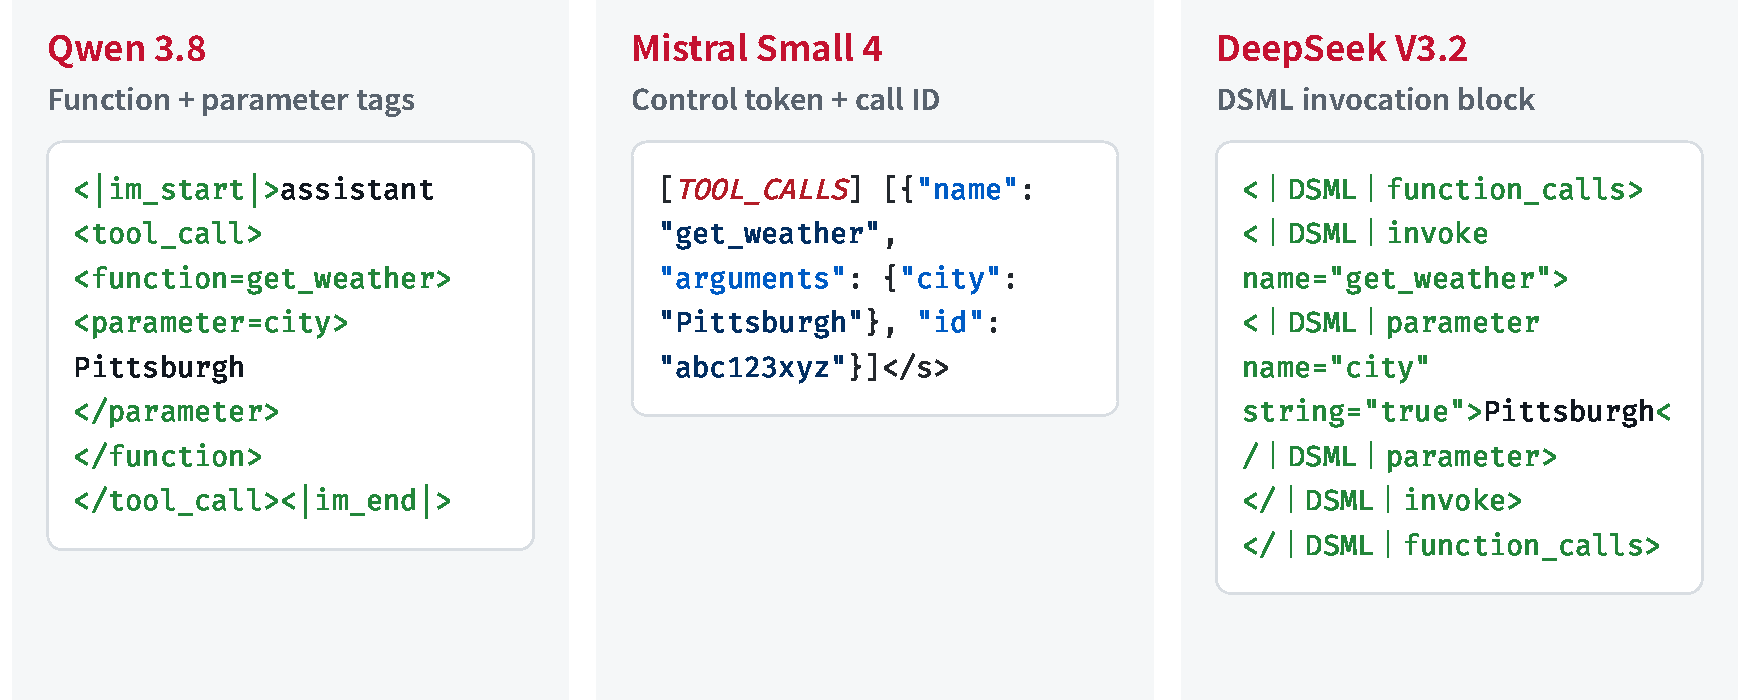
\includegraphics[width=1\textwidth]{figures/三种模型工具协议.pdf}
\caption{同一天气调用在三种模型协议中的序列表示。\protect\footnotemark}
\end{figure}
\footnotetext{官方课件第 23 页裁图；对应口述 00:20:44--00:22:03。}

\begin{importantbox}{使用模型实际训练过的格式}
从已有模型继续微调时，训练数据应匹配该模型的工具调用格式；推理输入和解析器也应匹配。Hugging Face 的 \texttt{apply\_chat\_template} 负责应用对应模型的模板。API 层结构相似，不意味着 DeepSeek 的输出解析器可以直接用于 Qwen。
\end{importantbox}

课堂强调理解模板这一层的实际作用：否则表面上 tools 已提交，底层却可能以模型不熟悉的序列输入；或模型输出正确的本族格式，应用却用另一套解析规则处理。这类失败应归因于协议不匹配。

\subsection{注册、解析、校验、执行分别承担什么责任}
模型给出调用后，harness 还需要知道对应哪段实际程序。课件用 OpenHands 风格的 dispatch 流程说明两阶段组织：初始化时解析工具 spec、配置 executor，建立名字到 ToolDefinition 的映射；每次调用时解析 \{name,args\}，查表找到工具，再构造并校验 action，交 executor 执行，返回包含调用 ID 的 observation。

\begin{center}
\small
\renewcommand{\arraystretch}{1.25}
\begin{tabular}{L{2.4cm}L{5cm}L{5.2cm}}
\toprule
阶段 & 需要回答的问题 & 典型失败 \\
\midrule
解析 & 输出能否转成 name 与 arguments？ & 格式损坏、协议不匹配 \\
查找 & 名字是否属于已注册工具？ & 生成了不存在的工具名 \\
参数校验 & 参数是否符合 action 定义？ & 必填项缺失、类型错误 \\
实际执行 & 合法请求在当前环境能否完成？ & Python 运行错误、工具自身失败 \\
结果返回 & 反馈是否关联到原调用？ & 缺失结果、调用 ID 不匹配 \\
\bottomrule
\end{tabular}
\end{center}

\begin{figure}[H]\centering
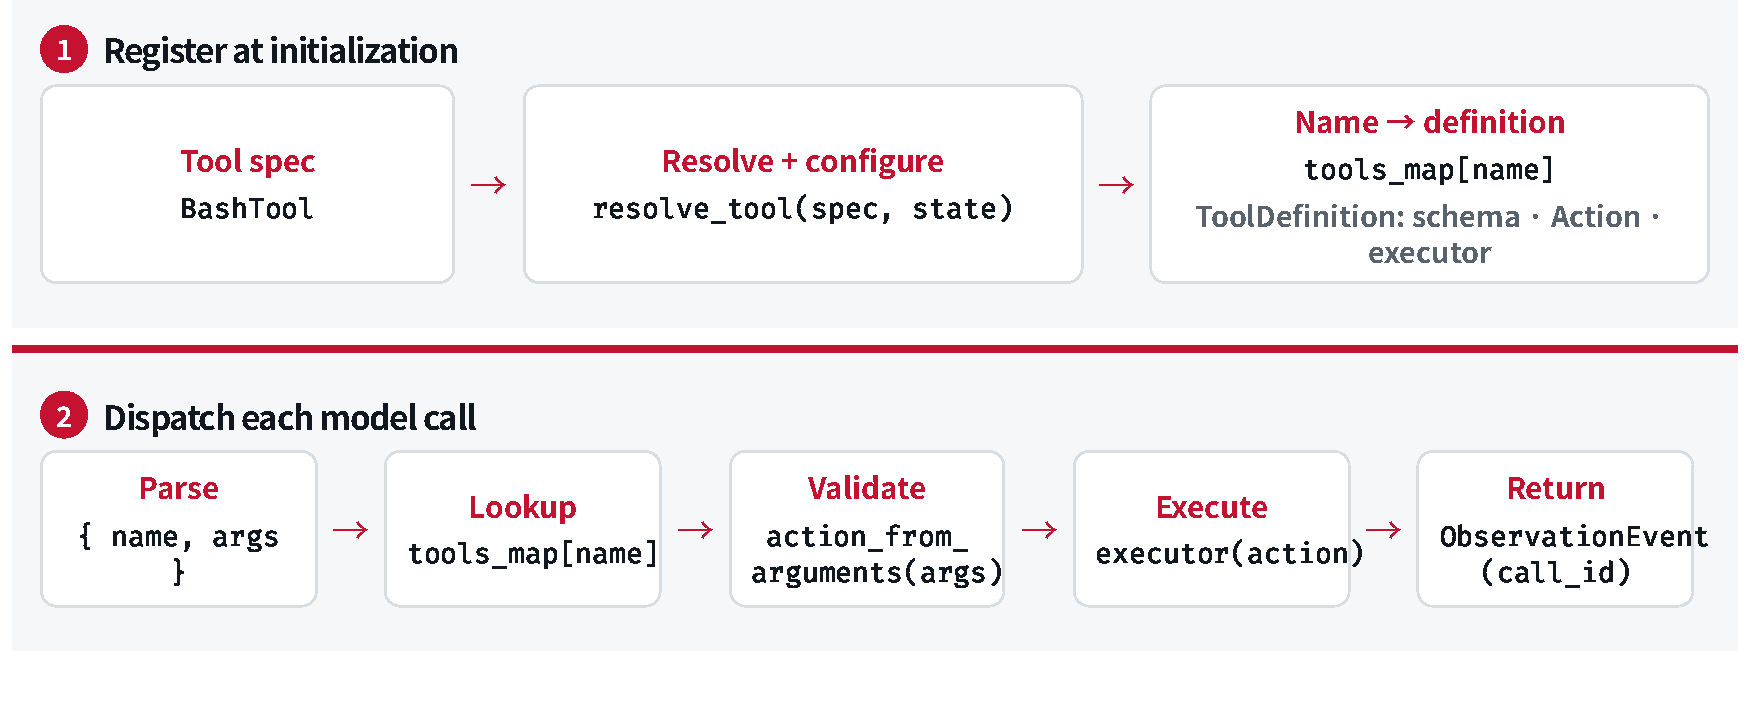
\includegraphics[width=1\textwidth]{figures/工具注册与派发.pdf}
\caption{初始化注册工具，运行时解析、查找、校验、执行和返回。\protect\footnotemark}
\end{figure}
\footnotetext{官方课件第 24 页裁图；对应口述 00:23:29--00:24:57。}

Python 执行工具解释了校验与运行失败的区别。参数接口可以接受一个字符串；字符串满足参数类型，不表示其中的 Python 程序一定能够执行。运行时仍可能报错。这样的错误也是观察，系统需要将它送回模型，后续行动才有机会依据实际失败调整。

\subsection{调用 ID 是历史完整性的一部分}
每次调用由模型推理层或 agent 代码附上 ID；结果消息携带匹配的 \texttt{tool\_call\_id}。当多个工具并行执行、返回先后顺序不同，ID 让每个结果仍能对应原请求。

\begin{figure}[H]\centering
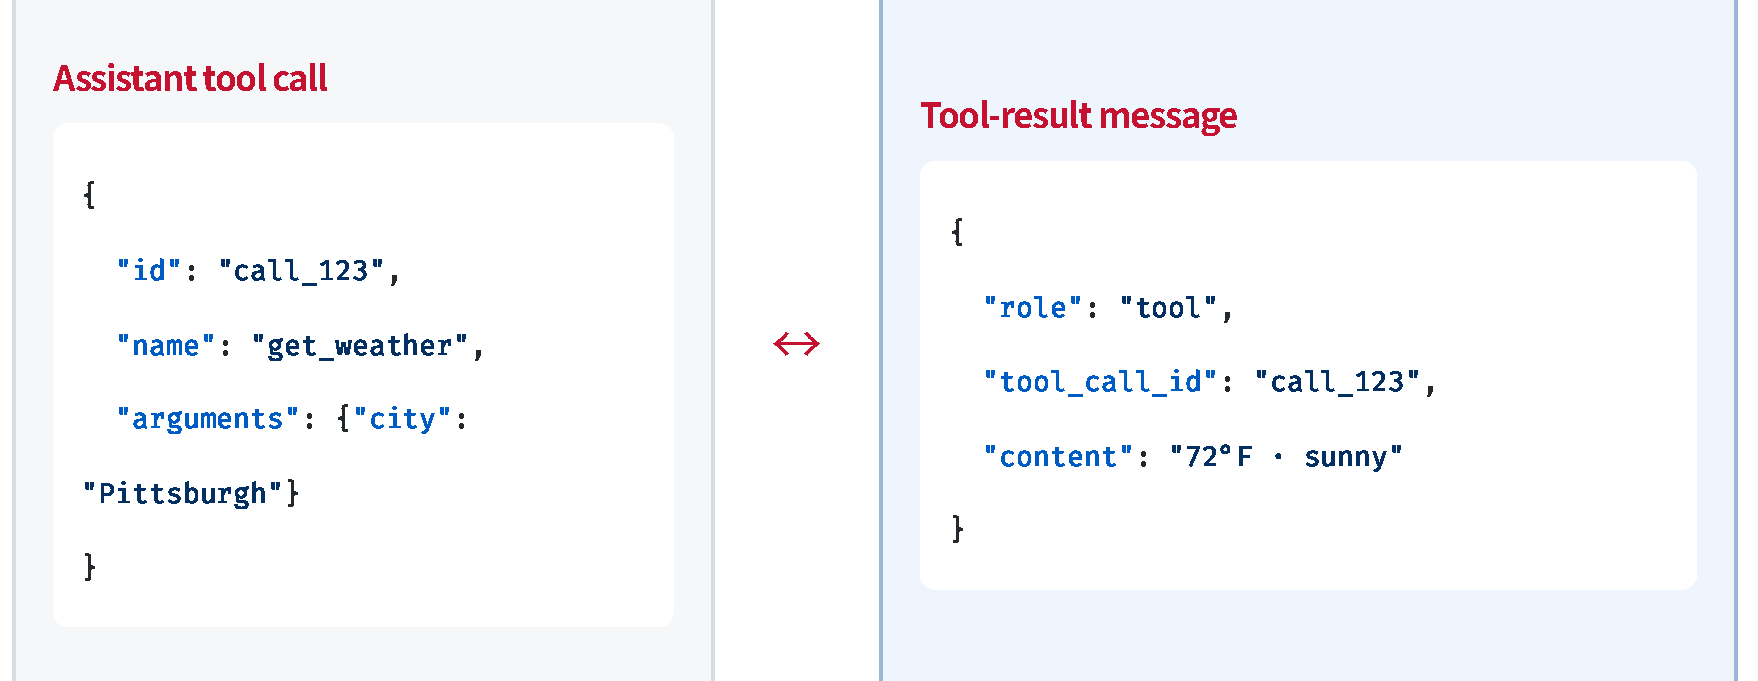
\includegraphics[width=.96\textwidth]{figures/调用与结果的ID.pdf}
\caption{调用对象与结果消息使用同一个调用 ID 建立对应。\protect\footnotemark}
\end{figure}
\footnotetext{官方课件第 25 页裁图；对应口述 00:24:57--00:26:47。}

讲者描述了实践中的恢复失败：assistant 调用已经写入历史，程序随后崩溃，结果尚未保存；恢复时历史留下没有对应结果的调用。有的服务会判定这段历史不合法并拒绝继续生成。这个例子说明，工具调用与结果写入之间还需要明确的恢复策略。具体协议行为取决于服务，但“恢复后的历史必须表达每次请求的实际状态”是可复用的系统要求。

\begin{warningbox}{重试时先查清调用是否执行过}
缺失结果不等于动作没有发生。对于产生副作用的动作，历史恢复应核对执行状态，再决定补记结果还是重试；盲目重试可能重复执行。这里是根据课堂崩溃案例作的工程展开，并非原课件给出的完整恢复算法。
\end{warningbox}

\subsection{本章小结}
消息、工具 schema 与模型 token 序列之间由模板连接。模型协议决定如何表达请求，harness 的 registry、校验器与 executor 决定如何执行；call ID 将真实反馈与原请求连接起来。模型输出、参数合法、实际运行和历史完整分别需要检查。

\clearpage
\section{约束解码：在生成时排除不合法的下一步}
\subsection{为什么仅在输出结束后解析还不够}
课件展示一个缺少闭合花括号的天气调用。模型的普通生成机制并不保证 JSON 正确；等生成结束后再解析，会抛出异常。讲者提到常见的事后补括号做法，但更系统的路线是将形式约束带入每一步解码，提前排除使输出不合法的候选。

约束包含不同层次。syntax 要求 JSON 可解析；shape 要求字段满足规定；types 要求 \texttt{city} 为字符串；values 要求温度单位属于允许集合。每层约束都能排除一种结构失败，却没有独立验证天气事实。

\begin{importantbox}{形式约束与任务正确性}
约束解码保证其所实现的格式规则。它不能保证模型选对工具、填入真实城市、获得权限或完成任务。一个结构完好的错误请求，仍然是错误请求。
\end{importantbox}

\subsection{JSON Schema 把接口要求变成机器可读规则}
天气接口要求 \texttt{city} 是字符串，\texttt{units} 只能为 C 或 F，\texttt{city} 必须出现，不接受额外字段。以下代码来自课件 schema 示例，保留了其规则；其中 units 未列入 required，因此此 schema 允许省略 units。

\noindent\begin{minipage}{\textwidth}
\begin{lstlisting}[language={},caption={天气参数的 JSON Schema：类型、必填字段、枚举与额外字段限制}]
{
  "type": "object",
  "properties": {
    "city": {"type": "string"},
    "units": {"enum": ["C", "F"]}
  },
  "required": ["city"],
  "additionalProperties": false
}
\end{lstlisting}
\end{minipage}

\texttt{\{"city":"Pgh","units":"F"\}} 和 \texttt{\{"city":"Pgh","units":"K"\}} 都是可解析的 JSON；后者违反 units 的枚举约束。K 是合理的温度单位，但此接口并不接受它。因此格式有效、schema 有效与现实语义合理，分别处于不同层次。

\begin{figure}[H]\centering
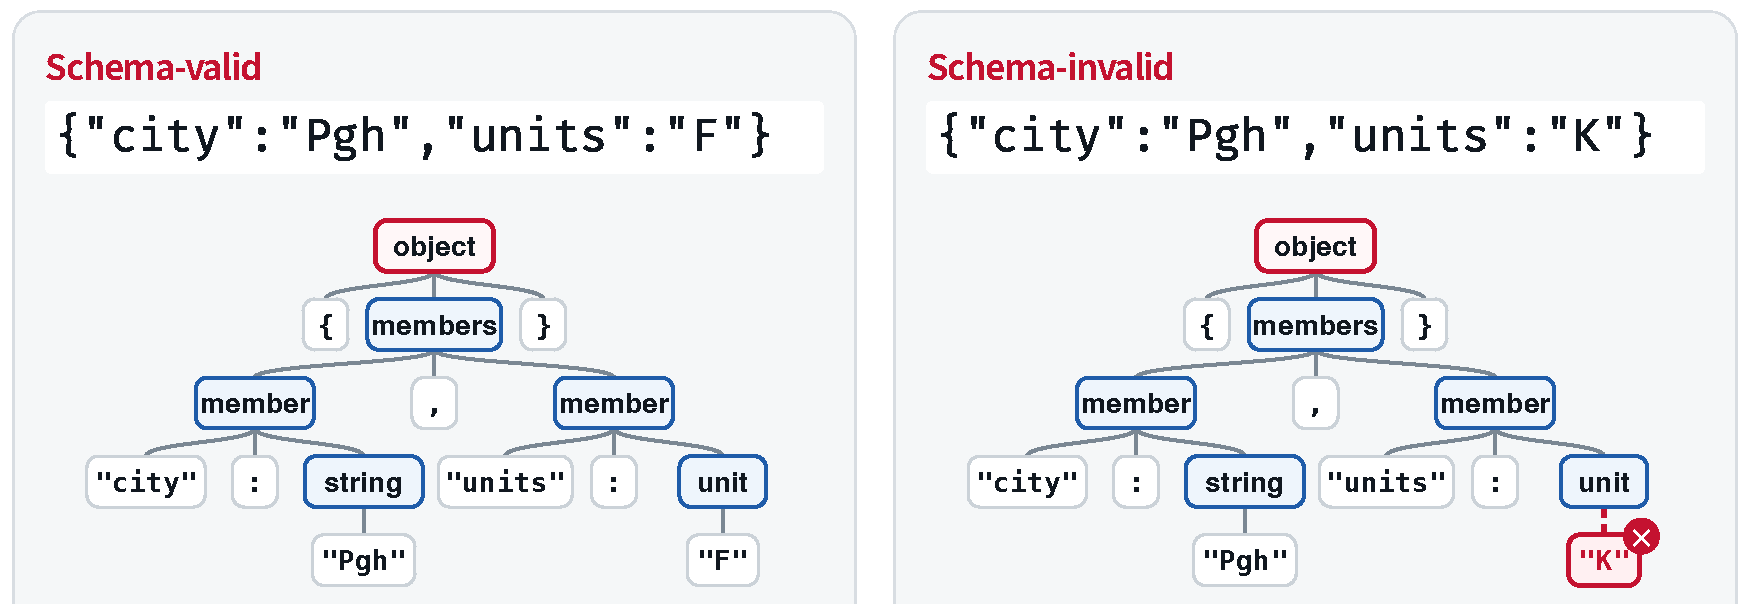
\includegraphics[width=1\textwidth]{figures/合法与非法语法树.pdf}
\caption{两个对象都能解析为 JSON，只有 F 满足本接口的单位枚举。\\{\footnotesize 官方课件第 30 页裁图；对应口述 00:30:47--00:31:21。}}
\end{figure}

\subsection{从有限状态到带栈的语法检查}
课堂从正则表达式和有限状态自动机引入形式语言：自动机读入符号，在有限状态之间转移，能表示正则语言。但 JSON 可以有任意深度的数组和对象嵌套；仅靠固定数量状态，无法一般性地记住每层括号该返回的位置。

上下文无关文法可描述这种递归结构，解析树展示对象、成员、键和值的组成。下推自动机（PDA）为有限控制增加栈：进入对象或数组时压入需要返回的上下文，闭合时弹出，继续处理外层规则。有限控制记录局部语法位置，栈记录嵌套层次及返回路径。

\begin{figure}[H]\centering
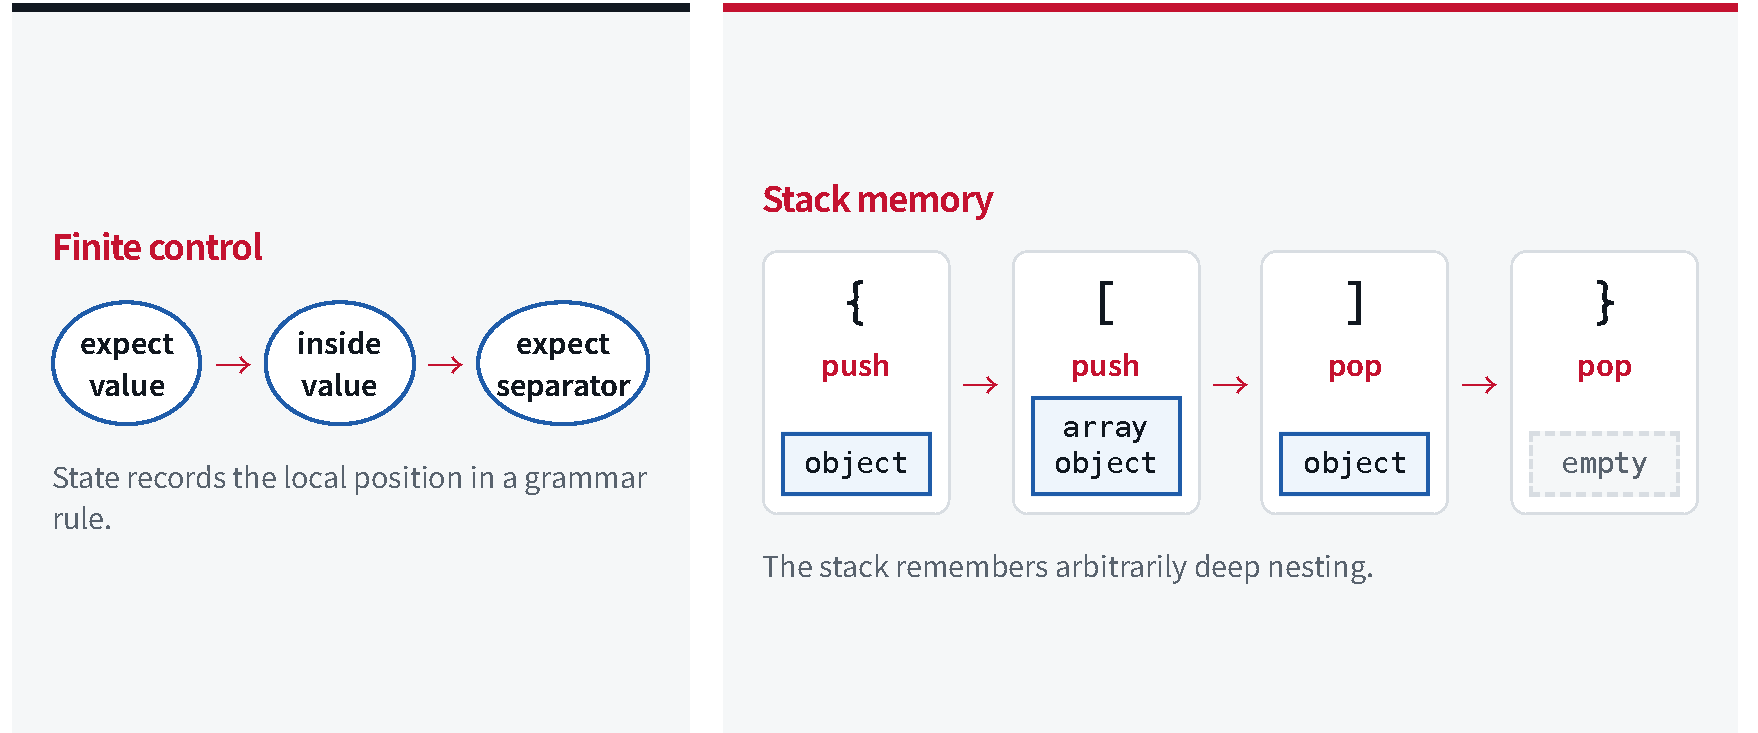
\includegraphics[width=1\textwidth]{figures/下推自动机的栈.pdf}
\caption{有限控制记录局部位置，栈记录嵌套对象与数组的返回路径。\protect\footnotemark}
\end{figure}
\footnotetext{官方课件第 31 页裁图；对应口述 00:31:21--00:33:31。}

\begin{knowledgebox}{本例可以用文法表达的范围}
递归 JSON 语法和本例的字段、类型、枚举限制可以组织成文法约束。这里不把整个 JSON Schema 规范的每一种语义校验都归为上下文无关文法；跨值比较等更一般规则是否受支持，需要看具体编译器与校验器。课堂机制的重点是利用支持的规则约束生成路径。
\end{knowledgebox}

\subsection{token 边界不会自动对齐语法边界}
官方讲义进一步说明：模型在 token 层预测，但语法检查需要处理候选 token 解码后的字节。一个 token 可能覆盖几个语法符号，也可能在字符串或其他语法单元中途结束。

课件例子假设某个候选 token 的文本为 \texttt{"F"\}}，其字节依次为十六进制 \texttt{22 46 22 7D}。它先完成字符串值，再闭合对象。PDA 必须让全部字节依次经过语法状态，才能判断这个 token 是否允许；不能只检查它的首字符，也不能假定一个 token 恰好对应一条文法终结符。这个例子用于解释边界问题，不声称每个 tokenizer 都有完全相同的 token。

\begin{figure}[H]\centering
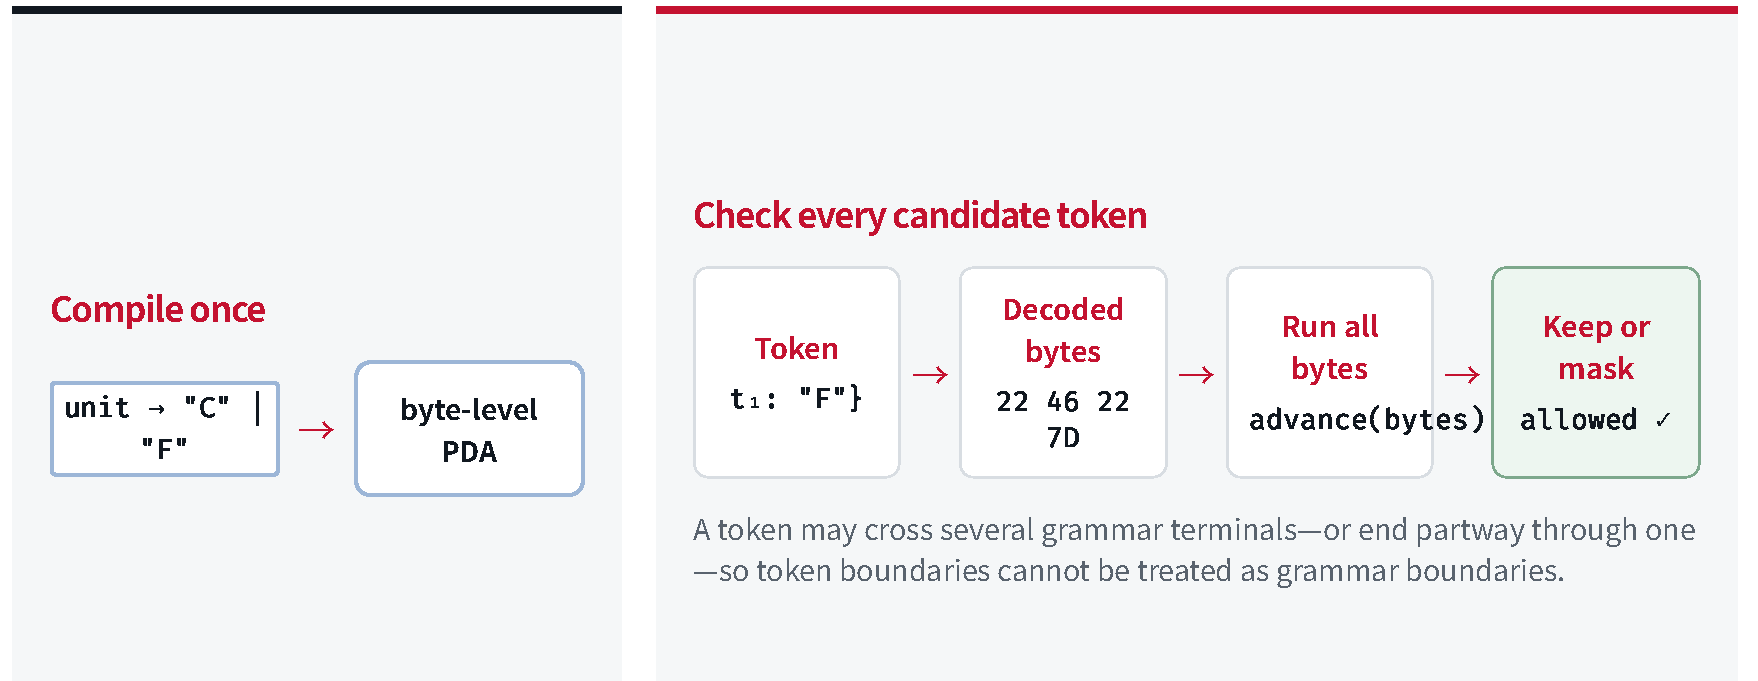
\includegraphics[width=1\textwidth]{figures/Token与字节边界.pdf}
\caption{官方课件补充：候选 token 需要按全部解码字节检查。\protect\footnotemark}
\end{figure}
\footnotetext{官方课件第 32 页；该页为当前官方课件中的补充展开，视频未展示此页。}

\subsection{mask 如何改变下一 token 的分布}
每一轮，模型先给出词表上所有候选的 logits。语法检查器根据当前已生成前缀，决定每个候选 token 是否能继续合法路径。允许的候选保留原分数，不允许的候选设为负无穷，再做 softmax。这样，非法候选获得零概率，合法候选之间仍按模型偏好采样。

以下是对课堂流程的数学重述，用于说明 mask 与重新归一化的关系：
$$
\widetilde z_t(v)=
\begin{cases}
z_t(v), & v\in A(s_t),\\
-\infty, & v\notin A(s_t),
\end{cases}
\qquad
p_t(v)=\frac{\exp(\widetilde z_t(v))}
{\sum_{u\in V}\exp(\widetilde z_t(u))}.
$$
\begin{itemize}
\item $t$：当前生成步。
\item $V$：模型候选 token 词表；$v$ 与 $u$ 是其中的候选 token。
\item $z_t(v)$：模型对候选 $v$ 给出的原始 logit。
\item $s_t$：语法检查器处理当前前缀后保存的状态；它可能包含多个匹配的栈配置。
\item $A(s_t)$：在当前状态允许的候选集合。
\item $\widetilde z_t(v)$：经过约束 mask 的 logit。
\item $p_t(v)$：mask 后归一化的采样概率。
\end{itemize}

该式假设当前存在至少一个允许候选。它不重新训练模型，也不增加对事实的认知；它直接在推理时修改可采样候选。若终止符也是候选，只有在符合完整输出的状态时才应允许正常终止。

\begin{figure}[H]\centering
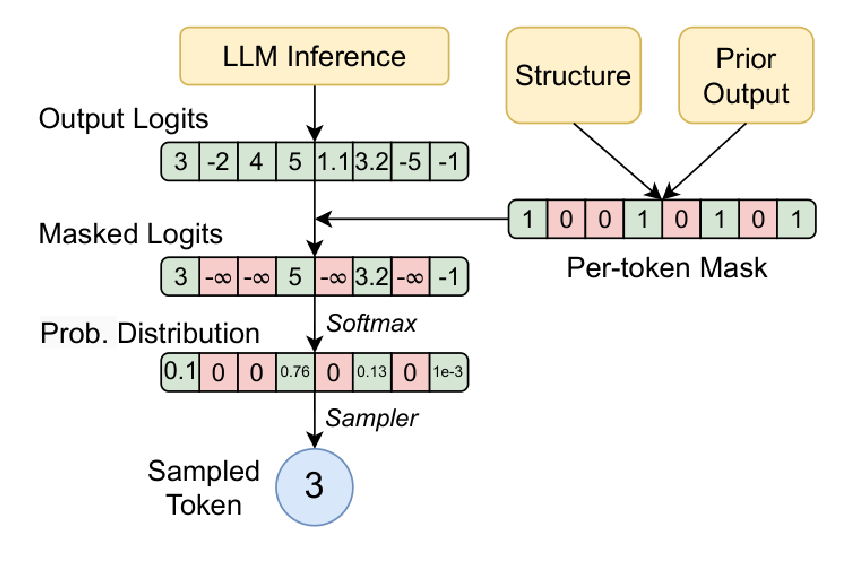
\includegraphics[width=.82\textwidth]{figures/Token掩码采样.pdf}
\caption{非法候选的 logit 被屏蔽，再归一化并采样。\protect\footnotemark}
\end{figure}
\footnotetext{官方课件第 34 页裁图，视频中为第 32 页；对应口述 00:31:21--00:33:31。}

\subsection{XGrammar 怎样减少每一步的检查成本}
直接为每个候选 token 重走全部栈状态，会增加解码成本。课堂用 XGrammar 介绍优化：在给定语法节点下，一大部分候选是否允许不依赖更深的栈，可以预计算并缓存；只有少数候选需要结合完整栈在运行时检查。

官方讲义将流程拆成四步。首先，按已生成字节推进匹配的 PDA 栈；其次，用栈顶语法节点取出缓存的允许或拒绝决定；随后，将依赖完整栈的少数候选做动态检查，并合并不同匹配栈的合法结果；最后合成完整 token mask，采样并更新栈。

\begin{center}
\small
\renewcommand{\arraystretch}{1.25}
\begin{tabular}{L{3cm}L{4.5cm}L{5.1cm}}
\toprule
优化机制 & 避免的工作 & 为什么仍需动态状态 \\
\midrule
语法节点的 mask 缓存 & 重复判断大量候选 & 少数 token 的合法性依赖深层栈 \\
持久执行栈 & 为不同解析分支反复复制整个栈 & 相同前缀可以共享，分支仍需独立演进 \\
CPU/GPU 工作重叠 & 将语法处理全部串行叠加到推理等待 & CPU 维护检查状态，GPU 运行模型，两者仍需同步候选与结果 \\
\bottomrule
\end{tabular}
\end{center}

这里的“上下文无关候选”是相对给定语法节点与栈状态依赖而言，不表示某个 token 在所有 JSON 位置永远合法。图中的绿色、红色部分代表已缓存的接受和拒绝决定，黄色代表需运行时检查的少数候选。持久栈支持共享解析前缀并保留分支；CPU 与 GPU 的工作重叠是该案例的系统优化，不意味着所有检查都自动免费。

\begin{figure}[H]\centering
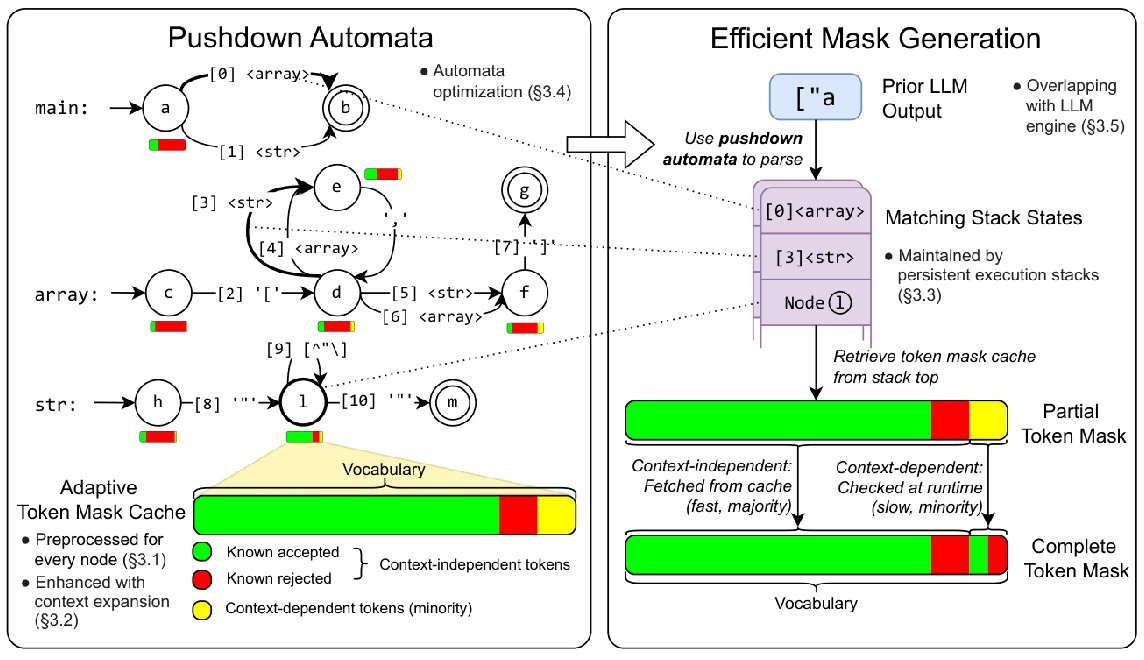
\includegraphics[width=1\textwidth]{figures/XGrammar_缓存与完整掩码.pdf}
\caption{XGrammar：缓存大部分候选，动态检查少数候选，并保留分支栈状态。\protect\footnotemark}
\end{figure}
\footnotetext{官方课件第 35 页裁图，原图来自 XGrammar；对应口述 00:33:31--00:34:27。}

下面的伪代码把决策顺序放在同一处，属于教学重写，未表达 XGrammar 的数据结构与实际 API：

\noindent\begin{minipage}{\textwidth}
\begin{lstlisting}[caption={教学伪代码：在每次采样前应用语法 mask},language=Python]
generated = list(output_prefix)
state = grammar.parse_prefix(output_prefix)
for _ in range(output_budget):
    logits = model.next_logits(generated)
    allowed = grammar.allowed_tokens(state)
    logits[~allowed] = -float("inf")
    token = sample(softmax(logits))
    generated.append(token)
    state = grammar.advance(state, token)
    emit(token)
    if token == EOS:
        break
\end{lstlisting}
\end{minipage}

其中 \texttt{allowed\_tokens} 概括字节级检查与缓存合并，\texttt{advance} 更新实际选中 token 对应的解析状态；\texttt{EOS} 的允许性也受 grammar 控制。该片段未展开无候选、异常、特殊 token 和预算耗尽处理，不能直接作为完整实现运行。

\subsection{合法前缀不等于已完成的 JSON}
课堂最后给出约束解码的边界：输出 token 预算耗尽时，模型可能沿合法路径生成了一部分 JSON，但尚未到接受终态。它没有选择非法下一步，却仍未生成可解析的完整对象。

\begin{warningbox}{检查完成状态，不能只检查每一步合法}
预算到达上限、请求被中断或输出被截断，都可能留下合法前缀。运行系统应区分“完整通过约束的输出”与“尚未闭合的中间状态”。讲者提出将剩余预算纳入约束是一种可能方向；本讲没有提供已经实现的算法。
\end{warningbox}

即使输出完整，schema 只规定 C/F 两种单位，也没有验证查询是否针对所需城市。形式检查应与参数语义、授权及真实工具结果验证共同使用。

\subsection{本章小结}
JSON Schema 描述结构要求，支持的规则可以进入文法检查；PDA 通过栈处理嵌套，候选 token 经字节级匹配形成 mask；mask 在采样前排除非法输出。缓存、持久栈与 CPU/GPU 重叠降低运行开销。保证成立的前提还包括输出正常完成，形式合法也仍需后续语义与任务验证。

\clearpage
\section{从库函数到远程工具：REST、OpenAPI 与 MCP}
\subsection{本地函数为什么还不是网络服务}
程序化工具调用可以让模型生成 Python，直接使用当前执行环境中的库。课件的天气库通过 \texttt{get\_weather(city,units)} 返回 \texttt{Weather}：名称、参数、类型与返回值组成进程内编程接口。

\noindent\begin{minipage}{\textwidth}
\begin{lstlisting}[caption={课件节选：进程内的天气库接口},language=Python]
from typing import Literal
from pydantic import BaseModel

class Weather(BaseModel):
    summary: str
    temperature: float

def get_weather(
    city: str,
    units: Literal["C", "F"] = "F",
) -> Weather:
    return provider.lookup(city, units)
\end{lstlisting}
\end{minipage}

这里 \texttt{provider} 是课件省略的天气提供方，不是一份完整实现。若远程应用也要调用它，还需要网络地址、传输协议、参数序列化和认证。函数已经存在，不表示它自动成为远程可访问的工具。

\subsection{FastAPI 把函数绑定到 HTTP 操作}
课件使用 FastAPI 将库函数暴露为 \texttt{GET /weather}。城市与单位来自查询参数，API key 从 \texttt{X-API-Key} header 获取；服务验证 key 后调用库函数，将 Weather 序列化为 JSON 返回。

\noindent\begin{minipage}{\textwidth}
\begin{lstlisting}[caption={课件节选：天气函数对应的 REST endpoint},language=Python]
from typing import Annotated, Literal
from fastapi import FastAPI, Security
from fastapi.security import APIKeyHeader
from weather_lib import Weather, get_weather

app = FastAPI(title="Weather API")
key_header = APIKeyHeader(name="X-API-Key")

@app.get("/weather", operation_id="get_weather")
def weather(
    city: str,
    key: Annotated[str, Security(key_header)],
    units: Literal["C", "F"] = "F",
) -> Weather:
    verify(key)
    return get_weather(city, units)
\end{lstlisting}
\end{minipage}

这个接口函数承担真实的网络边界：HTTP 参数绑定、key 获取、认证检查，以及库函数返回对象的序列化。\texttt{verify} 的具体实现未展示；声明 header 和认证方案不等于已经验证任何 key 都合法。

\begin{importantbox}{远程接口需要明确的访问契约}
请求包含 HTTP 方法与路径、query 参数和认证 header，响应包含 JSON 数据。模型负责提出所需工具与参数；harness 或客户端负责按网络契约发送请求，服务端实施实际认证与业务执行。
\end{importantbox}

\subsection{OpenAPI 描述操作，JSON Schema 描述值}
讲者指出 FastAPI 会自动生成机器可读接口说明，减少手写文档与 schema 的工作。官方课件把两个层次明确分开：OpenAPI 描述 HTTP 操作，包含路径、方法、\texttt{operationId}、参数位置和认证方案；其中嵌入的 JSON Schema 描述参数类型、枚举等值约束。

天气例子中的 \texttt{city} 在 query 中且为必填项；\texttt{units} 枚举为 C/F，默认 F；认证方案说明从 header 读取 \texttt{X-API-Key}。这些信息可用于构造 面向 Agent 的 工具定义，并在调用时映射为 HTTP 请求。

\begin{warningbox}{参数对象不包含整个 HTTP 契约}
仅知道 \texttt{city} 是字符串，不足以确定应该发到哪个地址、使用哪种方法、把参数放在哪里，以及如何认证。构造工具定义需要保留参数规则，工具执行器还需要正确实现 OpenAPI 所描述的网络契约。
\end{warningbox}

\subsection{Coding Agent 可以直接通过 shell 调用 REST}
如果 Agent 已经能够使用 shell，可以用 \texttt{curl} 请求 REST 服务。下面节选保留课件的查询编码与认证头：shell 展开环境变量，\texttt{curl} 将它加入 HTTP 请求。

\noindent\begin{minipage}{\textwidth}
\begin{lstlisting}[language=bash,caption={课件节选：用 curl 调用天气 REST 接口；示例域名并非可用服务}]
curl -sS -G https://weather.example/weather \
  --data-urlencode "city=Pittsburgh" \
  --data-urlencode "units=F" \
  -H "X-API-Key: $WEATHER_API_KEY"
\end{lstlisting}
\end{minipage}

这里的方便也带来清楚的访问边界：能够在同一 shell 中执行命令的 Agent，可能读取或误用该环境变量。把密钥藏在环境变量名后面，不等于从执行环境移除了它。

\subsection{MCP 统一发现与调用的接口}
MCP（Model Context Protocol）提供另一种 面向 Agent 的 接口。AI 应用作为 host，为不同服务器维护 client；服务器可以是本地 stdio 服务，也可以是远程 HTTP 服务。课程用天气服务和其他应用服务说明一个 host 连接多种能力的结构。

讲者起初认为，Agent 已经能调用普通 API，为什么还要多一层协议？随后讨论的重点是：MCP 统一了能力发现和调用契约，并可以在服务器边界中介上游凭证。它是暴露能力的一种选择，并非调用 REST 的必要步骤。

\begin{figure}[H]\centering
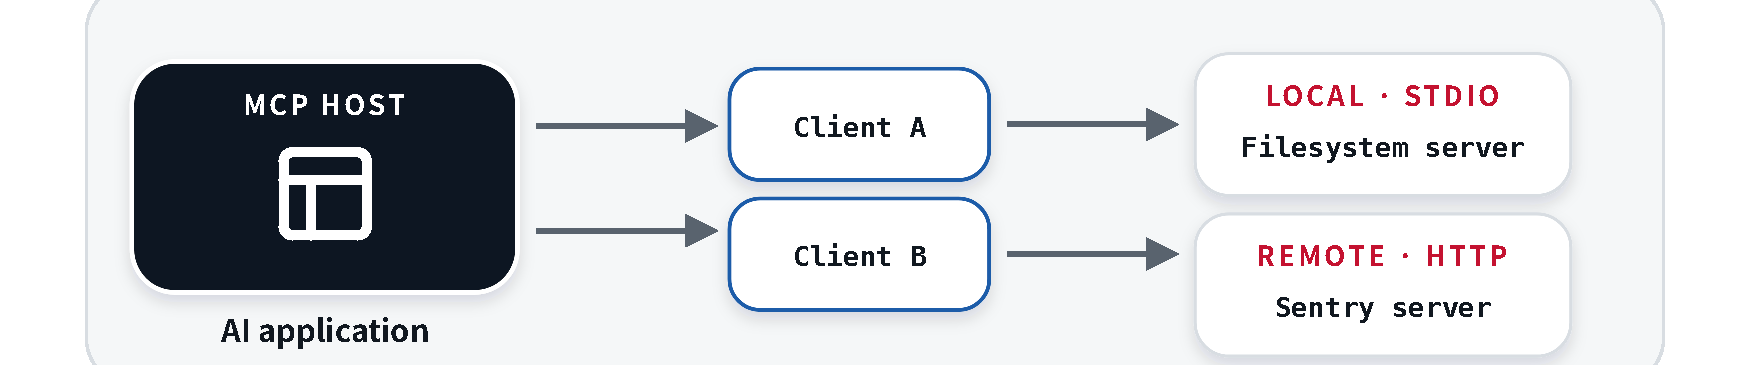
\includegraphics[width=1\textwidth]{figures/MCP主机与服务器.pdf}
\caption{一个应用通过多个 client 连接本地和远程 MCP server。\protect\footnotemark}
\end{figure}
\footnotetext{官方课件第 42 页裁图，视频中为第 40 页；对应口述 00:39:31--00:40:43。}

\begin{center}\small\renewcommand{\arraystretch}{1.25}
\begin{tabularx}{\textwidth}{L{2cm} X X}
\toprule
维度 & OpenAPI / HTTP API & MCP\\
\midrule
共同信息 & \multicolumn{2}{l}{名称、描述与结构化输入的 JSON Schema}\\
发现 & 获取 OpenAPI 文档 & 运行时调用 \texttt{tools/list}\\
调用 & HTTP 方法、路径与参数 & 经 MCP transport 调用 \texttt{tools/call}\\
认证 & 客户端向 HTTP API 认证 & 客户端向 MCP 认证；上游认证可独立管理\\
范围 & 描述 HTTP 操作 & 还支持 resources、prompts 和扩展\\
\bottomrule
\end{tabularx}\end{center}

讲者简要提到 MCP registry，可用于寻找已有服务器，本讲没有展开 registry 的治理或协议内部细节。

\subsection{FastMCP 将 OpenAPI 操作投影为工具}
课件通过 \texttt{FastMCP.from\_openapi} 演示把已有 OpenAPI 操作转为 MCP 工具：\texttt{GET /weather} 对应 \texttt{get\_weather(city, units)}。这种转换复用已有接口描述，底层工作仍由天气 HTTP 服务完成。

下面保留课件实现机制的关键行。原课件和视频的库名写作 \texttt{httpx2}；以下保留该课堂节选，用于说明服务器的凭证分离。\texttt{spec} 是已加载的 OpenAPI 文档；示例域名、库版本和外围初始化仍需具体环境提供。

\noindent\begin{minipage}{\textwidth}
\begin{lstlisting}[language=Python,caption={课件节选：从 OpenAPI 构造 MCP 工具与独立认证；展示凭证分离的接口机制}]
import os, httpx2
from fastmcp import FastMCP
from fastmcp.server.auth.providers.jwt import StaticTokenVerifier

upstream = httpx2.AsyncClient(
    base_url="https://weather.example",
    headers={"X-API-Key": os.environ["UPSTREAM_API_KEY"]},
)
mcp_auth = StaticTokenVerifier(tokens={
    os.environ["MCP_API_KEY"]: {"client_id": "course-agent"},
})
mcp = FastMCP.from_openapi(
    openapi_spec=spec,
    client=upstream,
    name="Weather MCP",
    auth=mcp_auth,
)
mcp.run(transport="http", port=8001)
\end{lstlisting}
\end{minipage}

该代码把两条认证连接分开：\texttt{UPSTREAM\_API\_KEY} 用于天气 API，\texttt{MCP\_API\_KEY} 用于保护 MCP 端点。课件指出静态 token 适合教学与开发，实际部署需要进一步设计和验证认证方案。

\subsection{认证边界：客户端与上游秘密分离}
在课程的设计中，Agent Harness 持有 MCP 访问凭证，MCP server 持有上游 API 凭证；模型可见的是工具信息与业务结果，不需要看到这两种秘密。客户端先 \texttt{list\_tools()}，再 \texttt{call\_tool("get\_weather", \ldots)}；服务器验证、授权、分派请求，并用自己的上游凭证访问天气 API。

\begin{figure}[H]\centering
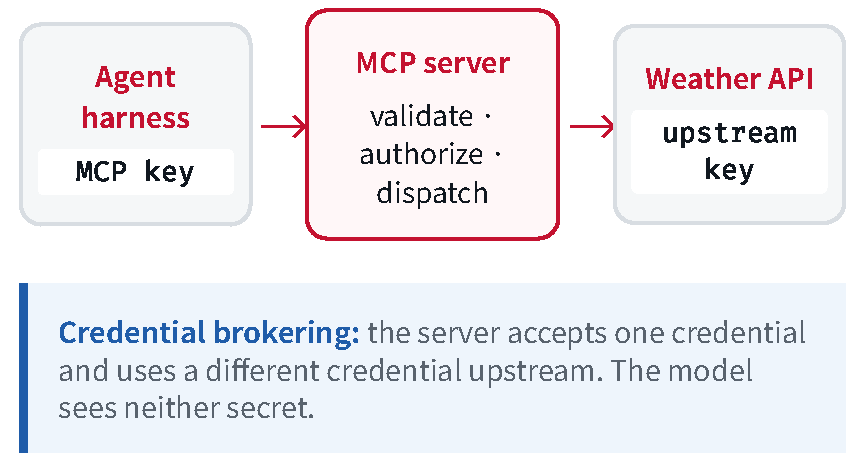
\includegraphics[width=.94\textwidth]{figures/MCP凭证中介.pdf}
\caption{MCP server 中介访问，在两个连接上使用不同凭证。\protect\footnotemark}
\end{figure}
\footnotetext{官方课件第 45 页裁图；相关口述 00:41:16--00:43:09。}

讲者用 GitHub token 泄露举例：如果原始上游秘密直接进入 Agent 能操作的环境，它可能被错误地写进公开仓库。服务器持有原始秘密、客户端只持有中介凭证，可以减少原始秘密暴露的范围。

\begin{warningbox}{凭证隔离的收益取决于权限设计}
讲者将 MCP 访问凭证描述为泄露后可能相对更有限的凭证。教学上应区分“没有暴露原始上游秘密”和“没有任何风险”：持有 MCP 凭证的人仍可能使用服务器授予的能力，损害范围取决于其权限。MCP 协议本身不会自动使秘密无害；本例的服务器分离与授权边界才产生隔离效果。
\end{warningbox}

课程还用一个小插曲指出接口表达能力的边界：天气可能同时晴与雨，讲者说演示中使用的天气 API 无法同时返回多个状态。这个例子说明接口可能因为建模过窄而丢失实际现象；它与前面的“形式正确不保证语义正确”相呼应。

\subsection{本章小结}
库函数、HTTP、模型 schema 与 MCP 分别描述不同层次的接口。REST 支持直接调用，MCP 支持统一发现、调用与凭证中介；运行系统负责请求构造、验证、授权和结果回流。

\clearpage
\section{并行工具调用：从多个请求到安全的并发执行}
\subsection{独立操作为什么不应逐次等待}
天气、日历和航班状态可以是互不依赖的查询。如果每次只生成一个调用，系统就反复经历“模型生成、工具等待、模型再生成”。课程的并行调用机制很直接：模型在一个响应中产生多个 tool call，Harness 同时发起这些独立操作，随后将所有结果带回下一轮。

\begin{figure}[H]\centering
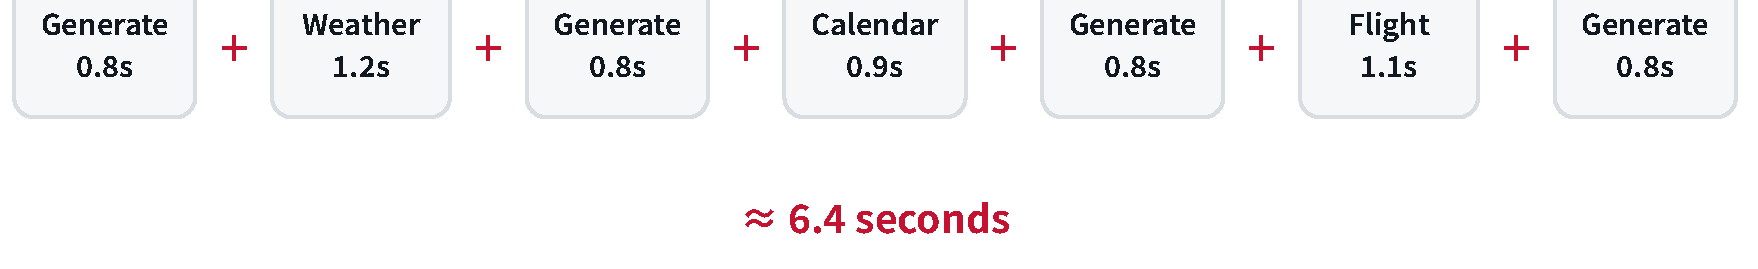
\includegraphics[width=1\textwidth]{figures/串行调用时延.pdf}
\caption{串行方案反复等待模型生成与工具完成。\protect\footnotemark}
\end{figure}
\footnotetext{官方课件第 48 页裁图；对应口述 00:45:16--00:46:04。}

\begin{figure}[H]\centering
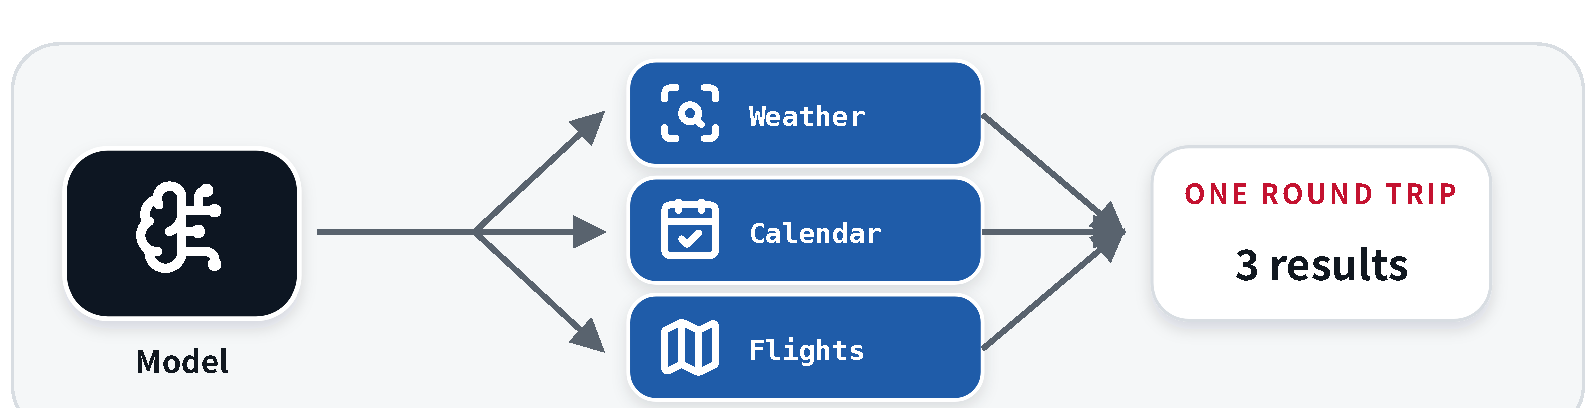
\includegraphics[width=1\textwidth]{figures/并行调用结构.pdf}
\caption{独立调用共享一次生成，等待后将三个结果带回下一轮。\protect\footnotemark}
\end{figure}
\footnotetext{官方课件第 49 页裁图；对应口述 00:45:16--00:46:04。}

\subsection{时延计算：等待总和变为最长等待}
课件给模型生成每次 0.8 秒，三个工具分别 1.2、0.9、1.1 秒。串行调用需要四次生成：三次提出调用，最后一次整理答案；并行调用需要一次产生全部调用，等待最慢工具，再一次整理答案。以下将课件数值推广为教学计数，忽略网络、调度和序列化的额外开销。
$$T_{\mathrm{serial}}=(m+1)g+\sum_{i=1}^{m}t_i$$
\begin{itemize}
\item $T_{\mathrm{serial}}$：串行方案的总时延。
\item $m$：独立工具调用的数量。
\item $g$：一次模型生成的时延，本例简化为相同值。
\item $t_i$：第 $i$ 个工具的执行时延。
\item $i$：工具索引，从 1 到 $m$。
\end{itemize}
并行方案共享一次调用生成和一次等待，等待时间由最慢工具决定：
$$T_{\mathrm{parallel}}=2g+\max_{1\leq i\leq m}t_i$$
\begin{itemize}
\item $T_{\mathrm{parallel}}$：并行方案的总时延。
\item $g$：一次生成的时延，前后两次生成贡献 $2g$。
\item $m$：独立工具的数量。
\item $t_i$：第 $i$ 个工具的执行时延。
\item $i$：工具索引；最大值取所有工具中最慢的一项。
\end{itemize}
代入课件数值，串行是 $4\times0.8+1.2+0.9+1.1=6.4$ 秒；并行是 $2\times0.8+\max(1.2,0.9,1.1)=2.8$ 秒。这是理想化对照，说明减少生成轮次与重叠等待的收益；实际时延还取决于网络与调度。

\subsection{依赖决定哪些调用可以并行}
课程给出一条必须串行的链：先找到 customer ID，再用 ID 查询订单，最后给选中的订单退款。后一步的参数来自前一步，无法在尚未取得结果时同时执行。天气、日历、航班的查询仅在任务本身没有把它们关联起来时才独立；如果航班操作取决于天气，也需要先获得天气结果。

\begin{importantbox}{并发许可比“没有数据依赖”更严格}
课件强调 independent, safely concurrent calls。没有参数依赖是一个条件，还需确认同时执行符合系统的访问与副作用约束。作为教学解释，同时写同一个资源即使参数各自已知，也可能产生冲突；独立只读查询更容易满足这些条件。
\end{importantbox}

\subsection{Harness 并发执行，调用 ID 关联结果}
模型一次发出多项请求，只说明表达了并行意图。实际是否重叠运行取决于 Harness。课件使用 \texttt{asyncio.gather}：为每个调用执行参数解析和工具分派，工具返回后带回 \texttt{call\_id}。

\noindent\begin{minipage}{\textwidth}
\begin{lstlisting}[language=Python,caption={课件节选：并发执行异步工具，并保留结果对应的调用 ID}]
async def execute(call):
    args = json.loads(call.arguments)
    value = await TOOLS[call.name](**args)
    return call.call_id, value

results = await asyncio.gather(
    *(execute(call) for call in function_calls),
    return_exceptions=True,
)
\end{lstlisting}
\end{minipage}

这是执行机制片段，依赖已经定义的 \texttt{TOOLS}、调用对象和异步工具。它展示并发等待，不代表为每项操作启动一个 CPU 线程。不同工具可能先后完成，反馈仍需对应正确的调用 ID。

\begin{knowledgebox}{异常与顺序的教学解释}
\texttt{gather} 收集结果的顺序与输入顺序对应，完成时刻可以不同。\texttt{return\_exceptions=True} 让失败作为结果项返回；失败项未必包含成功路径返回的 \texttt{(call\_id, value)}。真实 Harness 还需要识别异常并关联原调用、将失败转成模型可读反馈；课件没有在这里展开完整错误政策。
\end{knowledgebox}

\subsection{任务成本为何不能只看单次价格}
讲者认为，价格更高的模型有时反而有更低的每任务成本：它可能更快找到合适方案，也可能更好地将工具调用并行化。减少决策轮次、无效调用和执行时间，可能抵消单次生成的价格差异。这是需要按任务测量的经验判断，并不保证较贵模型总是更省钱。

在课堂问答中，讲者把并行行为的进步与强化学习中的效率激励联系起来：较强的任务时长或简洁性惩罚，会鼓励模型寻找更快的执行方式，并行独立工具就是其中一种。协议能表示多个调用与模型主动选择这种策略，是两个层次；有并行接口，不自动意味着模型会熟练使用它。

\subsection{本章小结}
并行调用减少反复生成与逐项等待，但需要同时满足依赖和安全并发条件。模型负责提出多项调用，Harness 负责真正调度并关联反馈。时延、轮次与任务成功应共同衡量，才能判断并发策略是否带来实际收益。

\clearpage
\section{评价工具使用：正确选择、执行结果与运营失败}
\subsection{BFCL 衡量什么}
工具调用能力是多步 Agent 的基础，但它不能独自证明完整 Agent 任务的质量。课程用 Berkeley Function Calling Leaderboard（BFCL）介绍评价的扩展：从单轮调用逐渐涵盖多轮、Agentic 工具任务和鲁棒性。课件引用 V4；这里保留课上的分类，分类用于说明本讲采用的评价设置。

\begin{center}\small\renewcommand{\arraystretch}{1.25}
\begin{tabularx}{\textwidth}{L{2.8cm} X}
\toprule
任务类 & 课件给出的内容\\
\midrule
Single turn & Simple、Multiple、Parallel、Multiple-parallel\\
Multi-turn & Base、Missing function、Missing parameter、Long context\\
Agentic & Web search、Memory\\
Robustness & Hallucination measurement、Format sensitivity\\
\bottomrule
\end{tabularx}\end{center}

模型是否幻觉出参数、格式变更是否改变表现，以及信息或工具缺失时如何继续，属于不同的评价设置。讲者明确区分这里的 tool-calling agents 与端到端 coding agents，不能把 BFCL 的某项分数直接当作真实软件开发成功率。

\subsection{四层评价需要不同证据}
课件把整套系统的评价分为选择、参数、轨迹和任务。它们对应的问题与证据并不相同：
\begin{center}\small\renewcommand{\arraystretch}{1.25}
\begin{tabularx}{\textwidth}{L{2cm} L{2.7cm} X L{2cm}}
\toprule
层级 & 要回答的问题 & 示例指标 / 失败 & 是否需执行\\
\midrule
Selection & 选对工具了吗？ & Precision / recall；漏调用或多调用 & 不一定\\
Arguments & 参数值正确吗？ & AST / schema match；字段或值错误 & 不一定\\
Trajectory & 顺序正确吗？ & Sequence success；依赖关系错误 & 通常需要\\
Task & 最终目标达成了吗？ & End-to-end success；答案可信却错误 & 需要\\
\bottomrule
\end{tabularx}\end{center}

选择与参数可以通过预期调用或结构匹配检查；真实执行才揭示环境是否接受操作以及任务是否完成。作为教学解释，接口合法、请求成功返回与满足任务目标仍是不同事件：一个类型正确的退款请求，可能指向错误订单；一个看起来合理的最终答案，也可能没有正确使用工具结果。

\subsection{正确性还需要效率、可靠性与安全}
正确的 Agent 可能因为太慢或太贵而无法实际使用。效率应观察延迟、调用次数、token 与成本；可靠性应观察超时、重试和部分失败；安全应观察政策、权限与副作用，并在对抗性输出和有实际后果的操作上测试行为。

讲者举出工具超时后能否恰当重试、工具不可用时能否选择替代方案，以及面对诱导错误使用工具的输出是否仍能遵守要求。这些是运行中的问题，不宜只用静态 schema 匹配评价。

\begin{importantbox}{诊断运营失败时区分责任层}
模型可能选错工具、填错参数或忽视结果；Harness 可能解析失败、认证错误、校验错误或错配 ID；服务商或工具可能超时、触发限流或执行报错。Production evaluation 需要基准准确率，也需要这些运行失败率。
\end{importantbox}

\subsection{同一模型名，服务表现仍可能不同}
课程展示 OpenRouter 的服务商工具调用错误率图。同一模型经不同 provider 提供，错误率存在明显差异。截图日期为 2026 年 8 月 27 日，可读的数值包括约 15.1\% 与低至约 0.01\% 的错误率。它是课堂展示的某时点观察，不能作为长期固定排名或未来服务质量保证。

\begin{figure}[H]\centering
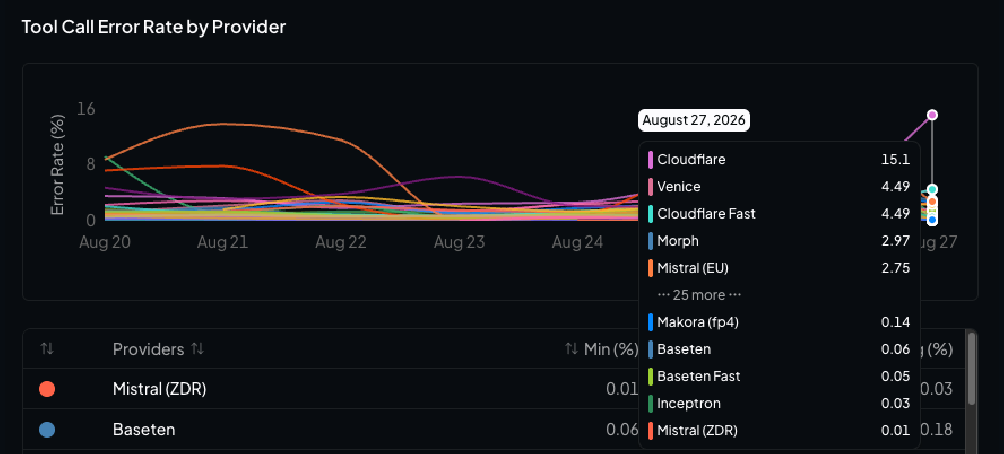
\includegraphics[width=1\textwidth]{figures/服务商调用错误率.pdf}
\caption{课堂展示的服务商错误率快照；图中提示框日期为 2026-08-27。\protect\footnotemark}
\end{figure}
\footnotetext{官方课件第 57 页裁图，视频中为第 55 页；对应讨论 00:51:51--00:55:37。}

讲者讨论了四种可能原因。第一，推理或解码实现不同；第二，量化程度不同，他的经验是 FP8 通常比更强压缩的 FP4 少一些错误调用；第三，speculative decoding 的实现可能不同；第四，语法约束解码的支持和算法不同。除此之外，服务本身也可能宕机或不可靠。

这些解释不能从一张 provider 曲线分别证明。量化是可能改变模型行为的因素，讲者对 FP8/FP4 的判断是个人经验。Speculative decoding 用较便宜的模型先预测较贵模型可能生成的内容，从而加速推理。对于这种机制，讲者特别区分无损和有损：无损方案应保持目标模型分布，不应因加速本身改变结果；有损近似则可能改变调用表现。不能将推测性解码一概写成错误率变化的必然原因。

\begin{warningbox}{模型名不等于完整部署配置}
工具使用表现来自模型、推理服务、约束解码、Harness 和实际工具的组合。比较 provider 时，还需知道测量定义、量化、服务配置与运行条件；课堂图证明的是差异存在，后续讨论给出待检查的原因。
\end{warningbox}

\subsection{本章小结}
评价从工具选择和参数结构出发，逐步检查轨迹依赖与最终目标；效率、可靠性、安全和 provider 运行条件决定这些能力在实际环境中能否发挥。静态匹配与执行评价互相补充，失败分类使改进能够落到具体层。

\clearpage
\section{总结与延伸：工具使用作为分层系统}
\subsection{讲者结束时保留的五层结构}
讲者在结束时将工具使用归纳为五层。能力层通过检索、执行、生成和应用操作扩展 Agent；机制层把 schema 放入提示，模型按协议发出调用，Harness 验证、分派并按 ID 关联结果；约束层用 JSON Schema 和 grammar masks 限制形式；接口层可选择直接 REST 或 MCP；系统层管理依赖与并发，并评价结果、成本和运营失败。

形式与语义的边界贯穿本讲。一个生成序列能被解析为 Python，不证明程序正确；一次 JSON 调用符合 schema，不证明工具适用；一次 HTTP 请求成功，不证明最终任务已达成。每一层都为后续层提供条件，最后仍需用环境反馈和任务标准检验。

\begin{figure}[H]\centering
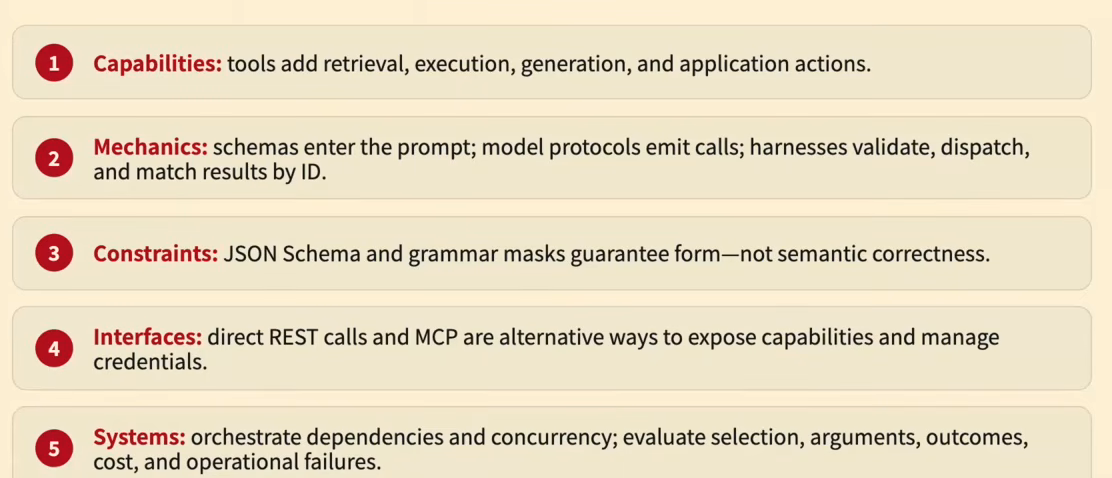
\includegraphics[width=1\textwidth]{figures/课程结束五层总结.png}
\caption{课堂最后完整呈现的五层总结。\protect\footnotemark}
\end{figure}
\footnotetext{视频画面对应字幕区间：00:56:08--00:56:43；截帧 00:56:40。}

\subsection{从调用链看清改进发生的位置}
下面是基于课程机制的教学归纳：工具描述决定模型知道哪些能力，模型行为决定何时选择和如何组合调用，约束解码限制输出形式，Harness 决定怎样执行和处理失败，工具与上游服务产生实际结果，评价判断完成程度。一次失败可以沿这条链定位，避免把所有错误都归于模型。

MCP 的凭证中介、并发的调用 ID、BFCL 的评价层次也沿同一条主线连接：接口要表达清楚的契约，执行要保留可靠的关联，评价要检查真实效果。更快的生成或更严格的格式都可能改善某一环节，但仍需要任务与运行证据判断总体收益。

\begin{figure}[H]\centering
\begin{tikzpicture}[node distance=7mm and 7mm, box/.style={draw=kbFrame,fill=kbBack,rounded corners,align=center,text width=3.35cm,minimum height=1.25cm,font=\small},>=stealth]
\node[box] (a) {消息与工具定义\\目标、历史、Schema};
\node[box,right=of a] (b) {模型生成\\选择工具与业务参数\\约束参与解码};
\node[box,right=of b] (c) {协议解析\\转换为结构化调用};
\node[box,below=of c] (d) {Harness 执行\\校验、权限、调度};
\node[box,left=of d] (e) {工具与服务\\本地程序 / REST / MCP};
\node[box,left=of e] (f) {结果与历史\\Observation、调用 ID};
\draw[->,thick] (a)--(b);\draw[->,thick] (b)--(c);\draw[->,thick] (c)--(d);
\draw[->,thick] (d)--(e);\draw[->,thick] (e)--(f);\draw[->,thick,color=kbTitle] (f)--(a);
\end{tikzpicture}
\caption{教学重绘：工具使用的一次完整交互；评价检查整条轨迹的效果与代价。}
\end{figure}

\subsection{实践要求与开放问题}
讲者说明，工具使用机制将用于第一次 Harness 作业：实现 Agent 时需要处理调用、执行和返回。下一讲转向长上下文管理，因为工具结果与轨迹会持续进入模型上下文；如何保留足够信息而控制成本，是这条闭环的下一个问题。

作为教学延伸，可以研究三个具体问题：在同一任务和 provider 下，约束解码减少了哪些格式错误，是否改变了语义错误比例？并行调用减少了多少生成轮次和等待，部分失败怎样影响任务完成？接口和凭证隔离怎样改变可用能力与泄露面？这些问题由本讲主题推导，课程未在本段给出实验结论。

\subsection{本章小结}
工具让 Agent 接触真实信息与操作，分层协议和运行系统使这些能力可调用、可约束、可观察。可靠工具使用需要把形式、语义、执行、并发和评价连接起来；这是构建 Harness 的基础，也是理解后续上下文管理的起点。
\subsection{来源与进一步阅读}
\begin{itemize}
\item 原视频：\href{https://www.youtube.com/watch?v=jXChFB4JSyw}{CMU AI Agents 2026: 2. Tool Use for Language Model Agents}，Graham Neubig。
\item 官方课件：\href{https://www.cmu-agents.com/slides/lecture-02-tool-use.pdf}{Tool Use for Language Model Agents}。图注页码对应本地保存的 60 页版本。
\item 带时间转录：\href{https://www.usetranscribe.io/yt/jXChFB4JSyw/ai-agents-tool-use}{公开课程转录}。术语、代码和图表结合视频与课件核对。
\item 工具综述：\href{https://arxiv.org/abs/2403.15452}{What Are Tools Anyway?}；程序化调用：\href{https://arxiv.org/abs/2402.01030}{CodeAct}。
\item 约束解码：\href{https://arxiv.org/abs/2411.15100}{XGrammar}；结构规范：\href{https://json-schema.org/draft/2020-12/json-schema-core.html}{JSON Schema Core}。
\item 工具使用评价：\href{https://gorilla.cs.berkeley.edu/leaderboard.html}{Berkeley Function Calling Leaderboard}。
\item 制作流程：\href{https://github.com/wdkns/wdkns-skills/tree/main/skills/youtube-render-pdf}{youtube-render-pdf}。
\end{itemize}

\end{document}
